%%
%% edengths.tex - LaTeX2e thesis driver
%%
%% Copyright (C) 1998 George Taylor
%% Copyright (C) 2010-2021 Mathew Topper <damm_horse@yahoo.co.uk>
%%
%% This file is part of the University of Edinburgh, Department of
%% Engineering LaTeX2e thesis template.
%% 
%%
%%   ABOUT
%%
%% This is the driver file for a Latex2e template which corresponds to the
%% regulations regarding layout of a thesis submitted within the University
%% of Edinburgh.

%%%% LOAD DOCUMENT CLASS

\documentclass[12pt,crest,nopardent,nosans,fancychap,hyper]{edengths}

%% Class options go in the square brackets above
%% i.e. \documentclass[options]{edengths}

%% Default report class options are:
%% (These are automatically included)
%%
%% a4paper
%% openright - Start chapters on righthand side pages
%% titlepage - Title should be on it's own page
%%


%% Standard available report class options are:
%%
%% 10pt
%% 11pt
%% 12pt
%% draft
%% final
%% fleqno
%% leqno
%% oneside
%% twoside

%% edengths class specific options:
%%
%% subsubnos - Enable numbering of subsubsections (note: these don't
%%             appear in the contents)
%% nosans    - Don't use sans serif fonts
%% nopardent - Remove paragraph indent and add a line skip
%% msfonts   - Use MS fonts rather than latex default
%% fancychap - Use fancy chapter headings like jthesis
%% crest     - Use a crest on the front page
%% labels    - Print labels in spine margin.
%% hyper     - Use the hyperref package to put clickable links into 
%%             the document. Use \autoref{fig:example} now instead of,
%%             say, figure~\ref{fig:example}. Settings are in
%%             edengfmt.tex.

%% ADDITIONAL FORMATTING can be done in 'edengfmt.tex' where the page
%% dimensions, header/footers, table of contents and the names of 
%% the bibliography and other formatting settings can be altered.
%% IN PARTICULAR THE LINE SPACING IS SET IN 'edengfmt.tex' AND
%% THE HYPERREF OPTIONS ARE SET HERE TOO. THIS SETS THE NAME OF
%% THE PDF, FOR EXAMPLE.

%% The class file should automatically detect pdflatex and provide
%% the right options.

%%%% LOAD USER DEFINED PACKAGES.

%% These are in ``packages.tex'' file and is automatically loaded
%% by the class file

%%%% LOAD USER DEFINED COMMANDS.

%%
%% defintns.tex - User defined commands for edengths.tex
%%
%% Copyright (C) 2010-2017 Mathew Topper <damm_horse@yahoo.co.uk>
%%
%%
%%   ABOUT
%%
%% This file contains the user defined commands for a Latex2e template which
%% corresponds to the regulations regarding layout of a thesis submitted within
%% the University of Edinburgh.

%%%%%%%%%%%%%%%%%%%%%%%%%%%%%%%%%%%%%%%%%%%%%%%%%%%%%%%%%%%%%%%%%%%%%%%%%%
%%%%%%%%%%             Define your commands here              %%%%%%%%%%%%
%%%%%%%%%%%%%%%%%%%%%%%%%%%%%%%%%%%%%%%%%%%%%%%%%%%%%%%%%%%%%%%%%%%%%%%%%%

%% New commands can be written using
%%    \newcommand{command}[inputs]{definition}.
%% In the definition the inputs are accessed with #1, #2, etc.
%%
%% If you want to override an existing command use \renewcommand instead
%% of \newcommand. \newcommand with give an error if command is already
%% defined.

%% If you are concerned that your command might override a default
%% you can use \providecommand which will ignore the new command if
%% a command of that name already exists.

%%%%% Some Example Maths Definitions (only use in maths mode)

\newcommand{\pdif}[2]{\frac{\partial #1}{\partial #2}}
%% ie \pdif{x}{t} would give partial x over t.

\newcommand{\dpdif}[2]{\dfrac{\partial #1}{\partial #2}}
%% inline partial derivative ie for $\dpdif{x}{t}$.
%% (\dfrac needs amsmath package)

\newcommand{\Ddif}[2]{\frac{D #1}{D #2}}
%% Material derivative

\newcommand{\spdif}[2]{\frac{\partial^{2} #1}{\partial #2^{2}}}
%% second partial derivative.

\newcommand{\altspdif}[3]{\frac{\partial^{2} #1}{\partial #2 \partial #3}} 
% mixed second partial i.e. \altspdif{x}{z}{t} = d2x / dzdt

\newcommand{\ndif}[2]{\frac{\mathrm{d} \, #1}{\mathrm{d} #2}}
%% ordinary differential.

\newcommand{\sndif}[2]{\frac{\mathrm{d} \,^{2} #1}{\mathrm{d} #2^{2}}}
%% ordinary second differential.

\newcommand{\me}{\mathrm{e}}
%% properly format Euler's constant, as opposed to variables called 'e'.
%% I do this because there is e.g. e_pool below

%%%%% Flux balance analysis

\newcommand{\epool}{e_{\mathrm{pool}}}
% enzyme pool variable

% (Works on Arch, but Ubuntu complains that these must be used in maths mode.
%  The `proper' way is to do \DeclareSIUnit, and I've done that in packages.tex)
%\newcommand{\mmolgdw}{\milli\mole~\gram_{DW}^{-1}}
%\newcommand{\mmolgdwh}{\milli\mole~\gram_{DW}^{-1}~\hour^{-1}}

\newcommand{\gro}{\lambda_{0}}
% growth rate, un-ablated

\newcommand{\Tiprop}{t_{\mathrm{par},i}}
% un-ablated/parallel/proportional time, component unspecified

\newcommand{\Tprop}[1]{t_{\mathrm{par},\mathrm{#1}}}
% un-ablated/parallel/proportional time, component specified

\newcommand{\Tiabl}{t_{\mathrm{seq},i}}
% ablated time, component unspecified

\newcommand{\Tabl}[1]{t_{\mathrm{seq},\mathrm{#1}}}
% ablated time, component specified

\newcommand{\biomfrac}[1]{f_{\mathrm{#1}}}
% biomass component fraction of dry cell mass, component specified

\newcommand{\griabl}{\lambda_{\mathrm{seq},i}}
% growth rate, ablated, component unspecified

\newcommand{\grabl}[1]{\lambda_{\mathrm{seq},\mathrm{#1}}}
% growth rate, ablated, component specified

\newcommand{\Tseq}{T_{\mathrm{seq}}}
% sequential time ('A')

\newcommand{\Tpar}{T_{\mathrm{par}}}
% parallel time ('B')

\newcommand{\ratioabl}{\tau_{\mathrm{seq}/\mathrm{par}}}
% ablation ratio

\newcommand{\exchrate}[1]{R_{\mathrm{#1}}}
% exchange rate of nutrient uptake


%%%% SET THE PATH FOR DIAGRAMS.

\graphicspath{
  {chapter_intro/}
  {chapter_methods/}
  {chapter_analysis/}
  {chapter_biology/}
  {chapter_model/}
}

%%%% PATH TO CREST

%% If you're not using the default crest files add the path here.
%% The default files are found in the 'front' directory.
%% Note: latex needs a eps file, while pdflatex needs pdf or jpg.
% \crestfile{/path/to/crest.pdps}

%%%% TITLE DETAILS

%% Author
\author{Arin Wongprommoon}

%% Title
\title{Single-cell time-series analysis of flavin-based yeast metabolic rhythms}

%% Qualification (Defaults to \textit{Doctor of Philosphy})
% \qualification{}

%% University (Defaults to \textsc{The University of Edinburgh})
% \university{}

%% Year of submission
\date{2023}

%% NOTE - IF YOUR USING hyper THEN THE ABOVE DETAILS NEED SET IN
%% edengfmt.tex AS WELL.

%%%% CHAPTERS TO INCLUDE

%% You may restrict which chapters are compiled using \includeonly
%% appendix/edengapp must be in the list if appendicies are included.

% \includeonly{front/frontmtr, chapter1/chapter1}
% \includeonly{chapter2/chapter2, chapter3/chapter3}
% \includeonly{chapter6/chapter6, appendix/edengapp,
%              appendix/appendx1 appendix/appendix2}

%%%% START DOCUMENT

\begin{document}

%%%% FRONT MATTER

\include{front/frontmtr}

%%%% START MAIN BODY TEXT

%% Call the edengths wrapper.
\startbody

%% The template will work with part definitions (starred or otherwise), but note
%% that nameref and autoref may not work properly for referencing them.
% TODO:
% - Editing
%   - Add/Read citations where marked
%   - Chemostat vs single-cell writing
%   - Reorganise end of flavins in YMC section
%   - Internal links/refs
% - Add figures & tables

\chapter{Introduction}

\section{Motivation of thesis}

This thesis aims to understand how an organism adapts its metabolism and cellular processes in response to external conditions.
I do so by through using the yeast metabolic cycle (YMC) as a framework for biological oscillators.
My reasons are twofold: (a) biological oscillators are important for coordination of responses and are present across kingdoms, (b) there are unanswered questions about the mechanistic basis of the YMC and about reconciling evidence from two types of experimental studies.
Therefore, I study YMC regulation in isolated cells in different nutrient conditions.

% - describe the logic of the rest of the chapters
% TODO: replace chapter numbers with \ref{}
This thesis is divided into six chapters:
\begin{enumerate}
  \item Chapter 1 discusses the background behind the yeast metabolic cycle and using flavin autofluorescence as a way to monitor the yeast metabolic cycle.
  \item Chapter 2 discusses the methods: single-cell microfluidics of yeast cells followed by an automated image analysis pipeline.
  \item Chapter 3 discusses the analysis of oscillatory time series; given the size of the datasets and the challenges of analysing noisy low-resolution time series, this deserves discussion in its own right.
  This chapter will step through the process of analysis and provide a review \& justification of the computational methods at each stage.
  \item Chapter 4 presents biological results, using the analysis methods discussed in chapter 3.
  I show that the metabolic cycle and cell division cycle are autonomous and synchronise in permissive conditions, while perturbations affect the relationship between these two biological oscillators.
  \item Chapter 5 discusses using flux balance analysis to answer whether temporal partitioning of biosynthesis under proteome constraints explains the timing of the yeast metabolic cycle.
  \item Finally, chapter 6 combines previous understanding of the metabolic cycle, experimental observations, and mathematical models to propose a coarse-grained, phenomenological model of the yeast metabolic cycle.
  This chapter also suggests further avenues of study.
\end{enumerate}


\section{Yeast metabolic cycle}
\label{sec:intro-ymc}

\subsection{Introduction to biological rhythms}
\label{subsec:intro-ymc-biological_rhythms}

\subsubsection{Biological basis of biological rhythms}
\label{subsubsec:intro-ymc-biological_rhythms-biological_basis}
% Physiological importance of biological rhythms
% including the circadian rhythm, cell division cycle, yeast metabolic cycle
% Basis, e.g. biochemical oscillators

% Literature:
% Mellor (2016) -- provides a good overview.
% and that collection of review articles probably give good definitions

[FIGURE: SHOW COMPONENTS OF A BIOLOGICAL OSCILLATOR, ADAPTED FROM MELLOR 2016]

Biological rhythms are repeating physiological or cellular processes.
Genetic oscillators, biochemical oscillators, and metabolic oscillators, all linked to a cellular redox cycle, govern biological rhythms \citep{mellorMolecularBasisMetabolic2016}.
Biological rhythms can occur at different time scales, from seconds (e.g.\ glycolytic cycle), to ultradian cycle (i.e.\ cycles that are more frequent than 24 hours), to circadian rhythms (24 hours).
Biological rhythms are important in temporally separating physiological processes.
This is instrumental in responding to external conditions, including nutrient conditions, growth requirements, or the day-night cycle.
Thus, this means that biological rhythms can vary according to conditions.

[FIGURE(S) MAY BE USEFUL IN DEMONSTRATING THE CELL DIVISION CYCLE HERE.  SHOW G1/S/G2/M PHASES, SHOW OVERVIEW OF CDKs, ETC.]

% VERY useful citation: adlerYeastCellCycle2022

Such biological rhythms include the circadian rhythm and the cell division cycle.
To demonstrate the definition of biological rhythm, I will discuss here the cell division cycle, which is well-characterised.
The cell division cycle in budding yeast is governed by a series of gene regulatory networks that interact in a feedback loop, resulting in oscillatory expression of regulatory proteins, namely, cyclin-CDK complexes that regulate cellular events in a temporal manner \citep{adlerYeastCellCycle2022, orlandoGlobalControlCellcycle2008, murrayRecyclingCellCycle2004}.
This cycle also includes biochemical and metabolic oscillators, for example, biosynthesis during S phase.
As with other biological rhythms, the cell division cycle also includes a system to control it, so that DNA replication occurs once every cell division cycle and so that the cell only divides when necessary.
The importance of such control systems are highlighted by disorders when these systems are impaired, such as chromosome aberrations and cancer.

The yeast metabolic cycle is a type of biological rhythm because it has the properties that define a biological rhythm.
Namely, it has gene-expression oscillators as evidenced by transcript cycling in its phases,
it has biochemical oscillators as evidenced by changes in dissolved oxygen in the chemostat,
and it has metabolite oscillations as evidence by changes in the levels of compounds that undergo redox reactions like NADH/NADPH and flavins.
I discuss further this evidence in the context of the known progression of the yeast metabolic cycle in section \ref{subsubsec:intro-ymc-definition-phases}.
However, in contrast to the cell division cycle, the control mechanisms of the yeast metabolic cycle are less well characterised --- I discuss this further in section \ref{subsec:intro-ymc-unresolved}.

\subsubsection{Theoretical basis of biological rhythms}
\label{subsubsec:intro-ymc-biological_rhythms-theoretical_basis}
% - Mathematics of systems of coupled oscillators.

% Single oscillations
% Useful here: cell division cycle modelling literature, e.g. Novak/Tyson,
% Adler et al. (2022) -- comprehensive review of cell division cycle models
% Goldbeter (2022) -- models of several examples
The theoretical basis of biological rhythms originated in work in the 1960s, which included simple systems of ordinary differential equations to describe negative feedback control circuits \citep{goodwinOscillatoryBehaviorEnzymatic1965, griffithMathematicsCellularControl1968}.
Experimental observations have then informed the development of models with finer detail.
Furthermore, synthetic genetic circuits have also been modelled and developed \citep{elowitzSyntheticOscillatoryNetwork2000}.

To illustrate a natural biological rhythm, I discuss the cell division cycle.
The well-characterised cell division cycle has inspired models with a variety of approaches.
Early models are based on a negative feedback loop of key components as identified by experimental studies.
For example, \textcite{goldbeterMinimalCascadeModel1991} assumed a minimal model of one cyclin, one kinase, and one protease to construct a negative feedback loop with a delay, giving rise to stable oscillations.
Such a strategy forms the basis of later models that incorporate more detail, including additional control points of the cell division cycle \parencite{chenIntegrativeAnalysisCell2004}, responses to perturbations such as osmotic stress \parencite{adroverTimeDependentQuantitativeMulticomponent2011}, and relationship with other oscillators like the circadian rhythm \parencite{gerardEntrainmentMammalianCell2012, charvinForcedPeriodicExpression2009, droinLowdimensionalDynamicsTwo2019}.
More recent, comprehensive models include \textcite{adlerYeastCellCycle2022} which is based on a system of ordinary differential equations adapted for the modelling to pheromone and osmotic shock responses, and \textcite{novakMitoticKinaseOscillation2022}, which models the cell division cycle as a series of switches between two stable steady states whose behaviour is regulated by the CDK oscillator.

In contrast, less well-characterised natural biological rhythms have given rise to models with fewer detail and precision.
An example is the glycolytic oscillation.
The glycolytic oscillation is a type of ultradian biochemical oscillator, characterised by oscillations in NADH levels (and other cofactors) in budding yeast cells at the time scale of 10-ish seconds \parencite{doddLiveCellImaging2017, lloydSaccharomycesCerevisiaeOscillatory2019, olsenOscillationsYeastGlycolysis2021}, when they are in high-glucose conditions.
A recent model is a coarse-grained model
driven by positive feedback loops as a system of two coupled instability-generating mechanisms \parencite{goldbeterMultisynchronizationOtherPatterns}.

% Forced oscillators, coupled oscillators
% Useful here: \textcite{tysonTimekeepingDecisionmakingLiving} and related reviews
As biological rhythms are often coupled with each other, forced and coupled oscillators have been modelled.
If an oscillator is forced, it has a natural oscillation frequency, but is forced from it due to an external force applied at a regular interval.
An example is the circadian clock, which is entrained to the light-dark cycle \parencite{goldbeterMultisynchronizationOtherPatterns}.
Yeast glycolytic oscillations can also be entrained via a periodic input of substrate.
Forced oscillators are closely linked to coupled oscillators, in which two oscillators are coupled to each other by certain activation/deactivation events.
Two coupled oscillators tend to oscillate at a compromise frequency if the natural frequencies of each are close enough to each other.
Otherwise, complex oscillations can occur: the oscillators lock to a rational ratio of frequencies --- i.e.\ one oscillator goes through $p$ periods while the other goes through $q$ periods.
In this case, the exact ratio depends on the ratio of the natural frequencies.
Furthermore, in certain cases, chaos can occur.
There is a mathematical basis in Arnold tongues \citep{heltbergTaleTwoRhythms2021}.
Experimental observations support this.
For example, \citet{charvinForcedPeriodicExpression2009} showed that externally forcing cell division cycles via glucose pulsing leads to phase-locking of the cell division cycle oscillator only within a range of extrinsic periods.

The yeast metabolic cycle has been modelled as a system of coupled oscillators \citep{papagiannakisAutonomousMetabolicOscillations2017,ozsezenInferenceHighLevelInteraction2019}, based on how it is linked to the cell division cycle.
I will discuss this in section \ref{subsec:intro-ymc-model}.

\subsection{Definition and description of the yeast metabolic cycle}
\label{subsec:intro-ymc-definition}
% Worth re-reading: Mellor 2016, Lloyd 2019

% Not too sure if the subsubsections in this subsection are a good idea.
\subsubsection{History of evidence for the yeast metabolic cycle}
\label{subsubsec:intro-ymc-definition-history}

Aspects of the YMC have been observed over decades.
\citet{nosohSYNCHRONIZATIONBUDDINGCYCLE1962} discovered that synchronised \emph{S. cerevisiae} cultures show oscillatory oxygen consumption.
\citet{kasparvonmeyenburgEnergeticsBuddingCycle1969} showed that gas metabolism and energy generation increase upon budding, while \citet{mochanRespiratoryOscillationsAdapting1973} described a high-amplitude respiratory oscillation following a substrate shift from glucose to ethanol.
\citet{satroutdinovOscillatoryMetabolismSaccharomyces1992} were the first to describe the metabolic components of a 40-minute YMC for cells in continuous culture.
\citet{tuLogicYeastMetabolic2005}
first incorporated transcript cycling in the description of the YMC and defined the YMC events,
based on a chemostat-based investigation of growth of budding yeast on glucose-starved conditions.

The yeast metabolic cycle is longer in duration and is more robust than a similar biological oscillator, the glycolytic oscillation.
The glycolytic oscillation has a period on the scale of 40 seconds \citep{olsenRegulationGlycolyticOscillations2009}.
In contrast, the yeast metabolic cycle has been described, using various definitions, to either exhibit a 40-minute short-phase cycle \citep{lloydUltradianMetronomeTimekeeper2005, liRapidGenomescaleResponse2006, lloydRedoxRhythmicityClocks2007}, or a long-phase cycle, which is most commonly described to be 4-5 hours \citep{tuLogicYeastMetabolic2005, tuCyclicChangesMetabolic2007}, but also ranges between 1.4 hours to 14 hours, depending on the chemostat dilution rate \citep{beuseEffectDilutionRate1998, oneillEukaryoticCellBiology2020}.

Glycolytic oscillations are highly damped, but yeast metabolic oscillations are robust, lasting for weeks \parencite{lloydRedoxRhythmicityClocks2007}.
Additionally, glycolytic oscillations have been observed in anaerobic conditions \citep{lloydSaccharomycesCerevisiaeOscillatory2019}, but yeast metabolic cycles have been observed in aerobic conditions.
Moreover, glycolytic oscillations are characterised by fluctuations in NADH fluorescence only, but yeast metabolic cycles consist of fluctuations in NADH fluorescence as well as fluctuations in other compounds like ATP and flavins.

\subsubsection{Phases of the yeast metabolic cycle}
\label{subsubsec:intro-ymc-definition-phases}
% INTEGRATE THIS STRUCTURE IN EACH PARAGRAPH THAT DISCUSSES EACH PHASE
% 1. Overarching theme of phase
% 2. Cellular events (cell division cycle, mitochondria)
% 3. Metabolic events (metabolite concentrations, redox)
% 4. Transcript/genetic events.
% Or any that make sense, e.g. 3 main events and all the evidence from different
% parts of biochemistry.
% Structure should then link well with the definition of biological rhythms in
% a previous subsection.
% ---------------------------------------------------------------------
Based on chemostat studies,
the YMC can be divided into two major phases: an oxidative, high-oxygen consumption (OX/HOC) phase and a reductive, low-oxygen consumption (RED/LOC) phase.
% Though Lloyd/Murray camp also describe these 3 phases
Many authors \citep{slavovMetabolicCyclingCell2011, murrayRedoxRegulationRespiring2011, caustonMetabolicRhythmsFramework2018} use oxygen consumption rates, evidenced by the change of dissolved oxygen concentrations over time, as a basis to refer to the YMC as a two-phase cycle.
Though, there are authors \citep{machneYinYangYeast2012} that base their two-phase model on the clustering of gene expression patterns.
\citet{krishnaMinimalPushPull2018} interpret the oxidative phase as a growth state, while the reductive phase is a quiescent state.
In contrast to the two-phase model, some authors identify a three-phase model with a reductive-building (RB) phase and a reductive-charging (RC) phase within the reductive phase, especially within the long-phase (4--5 hours) yeast metabolic cycle.
This three-phase model is primarily based on cellular events, including clustering of transcript trajectories \citep{tuLogicYeastMetabolic2005} and of metabolite concentration trajectories \citep{tuCyclicChangesMetabolic2007}.

Single-cell studies \citep{papagiannakisAutonomousMetabolicOscillations2017, baumgartnerFlavinbasedMetabolicCycles2018} do not discuss phases as the single-cell microfluidic set-up does not allow live monitoring of transcription, and oxygen consumption rate is an emergent property from chemostat cultures.
% ---- I don't think any publication explicitly says this -- it's mostly just Kevin IIRC.  I suggest phrasing it differently, below
%However, others [INSERT CHAIN OF PUBLICATIONS HERE] debate the existence of the reductive-charging phase and argue that this phase is an artefact of cellular adaptation to glucose limitation or feast-and-famine conditions.
Possibly, the two- or three-phase response results from cellular adaptation to glucose limitation in chemostat cultures, and it is unknown whether these dynamics hold true in glucose-rich conditions, which cannot be created in a chemostat \citep{slavovCouplingGrowthRate2011}.

[ADD DIAGRAM HERE -- MELLOR HAS A GOOD ONE, ADAPT HERS]

In the oxidative phase, cells consume oxygen at a high rate as respiration, fermentation, and
% Potentially may be the reason auxotrophs (hypothetically) don't have YMCs --
% but I showed that they do
energy-demanding processes
like biosynthesis and gene expression occur.
Occurrence of biosynthesis and associated gene expression is confirmed by increased transcripts from genes encoding components of the translation machinery and amino acid biosynthesis \parencite{tuLogicYeastMetabolic2005}.
As the oxidative phase transitions to the reductive phase, ethanol and acetate concentrations in the medium peak as respiration finishes \citep{tuLogicYeastMetabolic2005}.
`Redox state' metabolites, including NADH, NADPH, glutathione \citep{lloydUltradianMetronomeTimekeeper2005}, and flavins (FMN and FAD)
\parencite{murrayRedoxRegulationRespiring2011} become most oxidised in this phase.
Here, 70\% of metabolite concentrations peak with the combined autofluorescence of NADH and NADPH \citep{murrayRegulationYeastOscillatory2007}.

In the reductive phase, cells consume oxygen at a low rate.
During the reductive-building phase, activities linked to mitochondrial growth occur.
% as shown here.
There is evidence to suggest that activities linked to cell proliferation --- such as initiation of the cell division cycle, DNA replication, and spindle pole activity --- are gated to the reductive-building phase for both the short-period and long-period YMC.
Such evidence includes budding activity and the pattern of the expression of \emph{YOX1}, which encodes a cell division cycle repressor \citep{tuLogicYeastMetabolic2005}.

% There are many strings to pull on this phase.
Finally, during the reductive-charging phase,
non-respiratory metabolism and degradation processes occur to prepare the cell for the oxidative phase.
This non-respiratory metabolism includes glycolysis, ethanol and fatty acid metabolism, and nitrogen metabolism.
With these metabolic modes, under the regulation of the transcription factors Msn2p and Msn4p \citep{kuangMsn2RegulateExpression2017}, acetyl CoA accumulates so ATP can be produced in the oxidative phase \citep{tuLogicYeastMetabolic2005}.
After acetyl CoA levels reach a threshold, it promotes histone acetylation and thus induces the oxidative phase.
These metabolic pathways also optimise production of NADPH --- based on the induction of \emph{GND2} --- to buffer against oxidative stress in the oxidative phase.
Genes associated with protein degradation, ubiquitinylation, peroxisomes, vacuoles, and the proteosome also peak in the reductive-charging phase.

It has been hypothesised that gating activities linked to cell proliferation to the reduce-building phase
creates a temporal separation between oxidative biochemical processes (in OX) and the cell division cycle
This temporal separation may prevent reactive oxygen species generated by oxidative process from damaging DNA.
However, measuring DNA content and oxygen consumption in cells grown at different growth rates \citep{slavovCouplingGrowthRate2011} showed that the S phase of the cell cycle may occur in the oxidative phase if the cells have a slow growth rate.
% Not sure if they changed the growth rate of the cells though -- probably quite difficult
% to do in microfluidics setting.
% Re-phrase it a little to make it more different from Papagiannakis et al.
This may be explained by the YMC gating the early and late cell cycle independently, as evidenced by periodic localisation of the anaphase-promoting complex and mitotic exit activator Cdc14 phosphatase in metaphase-arrested cells \parencite{luPeriodicCyclinCdkActivity2010} and, conversely, the persistence of NAD(P)H cycling upon arresting of the late cell cycle by depletion of Cdc14 \parencite{papagiannakisAutonomousMetabolicOscillations2017}, all observed in single cells.
% What would be the function of such flexible gating?  Seems like community
% has no meaningful consensus yet.  Probably allocation of metabolites.
This evidence indicates that the gating between the YMC and the cell cycle is flexible.
Though there is no meaningful consensus as to the function of such flexible gating,
such gating can be instrumental in the allocation of metabolites to different temporal phases of both cellular oscillators.
% Discuss allocation of metabolites later -- and this can be linked to the modelling chapter of thesis.


\subsection{Yeast metabolic cycles under perturbations}
\label{subsec:intro-ymc-perturbations}
% - Nutrient perturbations
  % - Changing concentration or compositions of carbon sources.
  % - Changing concentration or compositions of nitrogen sources.
  % - Key deletion strains shed light on mechanism

Perturbations in growth conditions can affect the length of the metabolic cycle and its relationship with other cellular events.
The long-phase cycle may vary from 1.4 to 14 hours \citep{caustonMetabolicRhythmsFramework2018}.

\subsubsection{Perturbations in growth conditions}
\label{subsubsec:intro-ymc-perturbations-nutrient}

The main nutrient perturbations people have studied so far are perturbations in carbon sources and in nitrogen sources.

Perturbations in carbon sources are well-documented.
% change glucose concentration
Lower glucose concentrations prolong the metabolic cycle, as evidenced by both chemostat studies that assess the effect of changing the dilution rate \parencite{burnettiCellCycleStart2016, oneillEukaryoticCellBiology2020} and single-cell studies that assess the effect of glucose concentrations in the limiting region \parencite{papagiannakisAutonomousMetabolicOscillations2017}.
% 20 g/L --> 0.5 g/L doesn't seem to significantly prolong it, but maybe
% a greater effect will be seen if we get to the region of glucose limitation
% Though I am aware that this is my experimental observations -- need to see if literature confirms.
For example, decreasing the dilution rate decreases the growth rate, and in turn increases the duration of the oxidative phase relative to the reductive phases \citep{slavovCouplingGrowthRate2011}, thus prolonging the metabolic cycle.
This effect is pronounced in the region of glucose limitation.
Increasing the glucose concentration beyond a certain point does not produce an effect.
Additionally, several studies \citep{slavovCouplingGrowthRate2011,oneillEukaryoticCellBiology2020} show that the duration of the low oxygen consumption phase increases while the duration of the high oxygen consumption phase holds constant if the metabolic cycle duration increases due to these reasons.

Such experimental observations could by explained by models such as \textcite{jonesCyberneticModelGrowth1999}, which suggest that as the dilution rate is decreased, metabolic oscillations acquire greater amplitudes and longer periods, but if it low enough, metabolism becomes entirely oxidative, and metabolic oscillations disappear.
% ferm vs non-ferm
However, non-fermentable carbon sources like pyruvate give long-duration metabolic cycles in single cells, comparable to cells under limiting levels of glucose \parencite{papagiannakisAutonomousMetabolicOscillations2017}.

% bulk addition and depletion
In addition, bulk depletion or addition of a carbon source can reset the phase of the YMC.
Chemostat studies show that an initial starvation phase is needed to generate long-lasting synchronous metabolic cycles \parencite{tuLogicYeastMetabolic2005}. %[OTHER CITATIONS PROBABLY USEFUL].
On the other hand, adding a bulk carbon source such as acetate, ethanol, or acetaldehyde can reset the phase of the YMC \citep{kuangMsn2RegulateExpression2017, krishnaMinimalPushPull2018} or eliminate it \citep{jonesCyberneticModelGrowth1999}.

Perturbations in nitrogen sources are less well-studied.
% Maybe also because long OX stage as it's the stage for biomass building
\textcite{baumgartnerFlavinbasedMetabolicCycles2018}, based on single-cell observations, suggest that decreasing nitrogen source concentration prolongs the YMC, as evidenced by longer flavin oscillations when cells are grown on lower concentrations of yeast nitrogen base (YNB) media or on urea, a non-preferred nitrogen source.

In addition, perturbations outside nutrient sources also affect the YMC.
For example, externally applied hydrogen peroxide, as a source of oxidative stress, shifts the YMC to the oxidative phase \citep{amponsahPeroxiredoxinsCoupleMetabolism2021}.
% [MOVED FROM PREVIOUS SECTION]
Additionally, the oscillation period is insensitive to temperatures from \SI{25}{\celsius} to \SI{35}{\celsius} and media pH values from
2.9 to 6.0 \citep{lloydUltradianMetronomeTimekeeper2005} --- though the period of dissolved-oxygen oscillations decrease as pH decreases to below 2.9 and the oscillations disappear when conditions are too acidic \citep{oneillEukaryoticCellBiology2020}.

Finally, the phase difference between the YMC and cell cycle varies in different conditions % how?
% Confirmation that the YMC responds to nutrient availability?  How does phase
% resetting help the Cell Division Cycle then?
\citep{ewaldYeastCyclinDependentKinase2016}. % ok, but have I seen this phase shift with the different media (i.e. SC vs SM)?  What did Ewald have to say about this phase shift??
% 'bulk carbon source' -- could be adaptation to changing nutrient concentrations in general?
%Furthermore, the YMC can oscillate multiple times per cell cycle, or even disappear in some conditions \citep{baumgartnerFlavinbasedMetabolicCycles2018}. % which conditions?  can these be tested?
% --> also see Causton et al. (2015)
% -----------------------------------------------------------------------------------------------

\subsubsection{Genetic perturbations}
\label{subsubsec:intro-ymc-perturbations-genetic}

Although the molecular basis of the yeast metabolic cycle is not well-characterised, gene deletions shed light on it.
% Mellor (2016) provide an awesome table.
Genes that control the cell division cycle and metabolism have been deleted in studies.

Several deletions have been shown to remove the metabolic oscillations in chemostats: \emph{ZWF1} \citep{tuCyclicChangesMetabolic2007}, \emph{GSY2}, and \emph{GPH1} \parencite{oneillEukaryoticCellBiology2020}.
\emph{ZWF1} codes for glucose-6-phosphate dehydrogenase and is thus responsible for entry into the pentose phosphate pathway and subsequently a major source of NADPH generation, so deleting this gene may impair control of cellular redox.
However, because of its role, this gene deletion impairs adapting to oxidative and pH stress and also causes methionine auxotrophy, so it may be difficult to draw conclusions from this deletion in particular.
Furthermore, other enzyme-catalysed reactions in the cell that generate NADPH exist (Idp2p, Ald6p) and have shown to compensate for the loss of \emph{ZWF1} when cells are grown on lactate plates or on liquid cultures with glucose as the carbon source \parencite{minardSourcesNADPHYeast2005}.
This therefore raises the question of just how important \emph{ZWF1} is to the yeast metabolic cycle, and to what extent is NADPH generation is needed for control of cellular redox.
On the other hand, \emph{GSY2} and \emph{GPH1}, both have roles in glucose/glycogen mobilisation and storage.
The absence of dissolved oxygen cycles in these deletions thus suggest that cycling of carbohydrate stores may be needed for the function of the metabolic cycle.
However, metabolic oscillations have been observed in high-glucose conditions \parencite{papagiannakisAutonomousMetabolicOscillations2017, baumgartnerFlavinbasedMetabolicCycles2018} in which glycogen synthesis is repressed, therefore suggesting that glycogen cycling may play a more minor role in defining the yeast metabolic cycle and another nutrient cycling phenomenon may be more responsible.
In addition, \emph{MSN2} and \emph{MSN4} have been shown to regulate acetyl CoA accumulation in the reductive-charging phase, as evidenced by the lack of YMCs in deletion strains \citep{kuangMsn2RegulateExpression2017}.
This tells us that genes involved in signalling pathways play an important role in the integrity of the metabolic cycle too.

Additionally, other deletions have been shown to change the frequency or shape of dissolved oxygen cycles.
\textcite{caustonMetabolicCyclesYeast2015} provide several examples, of which I discuss \emph{RIM11}, \emph{SWE1}, and \emph{TSA1 TSA2}. % they actually had more, but these are the three that pop in my head right now
Rim11p is the yeast homolog of the GSK3$\beta$ serine/threonine kinase, which regulates metabolism and plays a role in setting the speed of the circadian clock.
The \emph{RIM11} deletion has been shown to result in shortened periods of dissolved-oxygen metabolic cycles in the chemostat, thus pointing towards a common mechanism for both biological oscillators.
Swe1p is a conserved cell division cycle regulator that functions at the G2/M checkpoint and has roles in coupling the cell division cycle with the circadian rhythm.
Deleting \emph{SWE1} also resulted in shortened periods of dissolved-oxygen metabolic cycles but with the same rate of DNA replication, suggesting a dysregulation in the coupling between the yeast metabolic cycle and the cell division cycle.
Tsa1p and Tsa2p are paralogous cytoplasmic thioredoxin peroxidases that cooperate in the peroxiredoxin-thioredoxin system to eliminate reactive oxygen species and have been shown to be a marker for circadian rhythms.
A double deletion of the two associated genes still results in metabolic cycles, but with an additional burst in high oxygen consumption during what would otherwise be the reductive-charging phase, showing that the peroxiredoxin-thioredoxin system is instrumental in the integrity of the yeast metabolic cycle.
In addition, \textcite{amponsahPeroxiredoxinsCoupleMetabolism2021} show the presence of cycling peroxiredoxin oxidation during the YMC using chemostat-based studies, with a corresponding cycling of hydrogen peroxide.
They also confirm that inactivating peroxiredoxins (tsa1$\Delta$ tsa2$\Delta$, additionally with inducible degradation of Ahp1, another cytosolic peroxiredoxin) disrupts the metabolic cycle and decouples it from the cell division cycle.
%Moreover, deletion of \emph{GTS1} shortens the oscillation periods \citep{lloydUltradianMetronomeTimekeeper2005},
Taken together, these deletion studies show that regulators of other biological rhythms and of redox metabolism play a role in the regulation of the YMC.

However, few genetic perturbation studies have been attempted in single-cell studies.
The most significant is in \textcite{baumgartnerFlavinbasedMetabolicCycles2018}, in which by deleting genes (atp5$\Delta$, cyt1$\Delta$) required for respiration, they showed that metabolic cycling does not require respiration.

\subsection{Modelling the yeast metabolic cycle}
\label{subsec:intro-ymc-model}

[THE SUMMARY FIGURES FROM THESE PAPERS MAY BE USEFUL TO HELP ILLUSTRATE THE IDEAS]

Mathematical models have been developed to explain the aspects of the YMC.
An early model is \parencite{jonesCyberneticModelGrowth1999} which simulates dynamic competition between three modes of metabolism --- fermentation, glucose oxidation, and ethanol oxidation --- using differential equations.
This model predicts spontaneous generation of oscillations in dissolved oxygen, cell mass, and storage carbohydrates in continuous cultures.
This prediction is consistent with chemostat-based studies of the yeast metabolic cycle.
Furthermore, the model predicts that, within a window of dilution rate values, if the dilution rate decreases, the dissolved oxygen oscillations increase in amplitude and period.
The increase in period agrees with experimental studies such as \textcite{oneillEukaryoticCellBiology2020}.
However, the model also predicts oscillations in the extracellular concentrations of glucose and ethanol, which conflicts with the steady-state assumption of chemostat studies.

\textcite{krishnaMinimalPushPull2018} uses a frustrated bistability model to produce a relaxation oscillator that explains how a population of yeast cells switches between quiescent and growth states when faced with a limited amount of metabolic resources.
This model assumes that the cells retain hysteresis of their current state and posits that cells of two populations communicate through diffused acetyl-CoA to sustain the population-level oscillatory behaviour.
Read together with the discussion from \textcite{burnettiCellCycleStart2016}, which also propose that yeast cells committed to the metabolic cycle secrete metabolites that induce other cells to enter the metabolic cycle provided that they have enough storage carbohydrates, this model provides an attractive cell-to-cell signalling explanation for the population-level behaviour observed in the chemostat.
However, such an explanation does not explain the presence of metabolic cycling in single-cell conditions in which cells are physically separated and signalling between cells cannot occur -- though it must be noted that autonomous generation of metabolic cycles and synchrony of metabolic cycles in a population can possibly arise from two different mechanisms that are independent of each other.

Based on single-cell experimental observations, \citet{ozsezenInferenceHighLevelInteraction2019} use a deterministic Kuramoto model to explain the interaction between one metabolic oscillator and three cell cycle oscillators at different stages.
This study builds upon use of the Kuramoto model to model collective oscillatory behaviour in other biological systems.
The study uses growth on different carbon source conditions to determine parameters that define the natural frequencies of the cell division cycle oscillators and the strength of the coupling between the four oscillators.
Parameter optimisation predicts that the metabolic cycle most strongly influences the START point of the cell division cycle, and more weakly influences the M and S phases, while the three points of the cell division cycle negligibly influence each other.
Under perturbations, the model system also exhibits stability but also a shift in oscillation frequency, agreeing with experimental observations, and also predicts the effects of Cdc20 and Cdc14 dynamic depletions.
However, a key criticism of this model-based study is that by using the Kuramoto model, it makes simplistic assumptions about the oscillators, which may be unrealistic especially given how little is known about the mechanistic basis of the metabolic oscillator.

% [This is a bit out of place... probably nix it given that I've given up on using this.]
% Additionally, a data-driven stochastic modelling approach was used to describe the relationship between the circadian and cell cycle oscillators without assuming a prior relationship \citep{droin_low-dimensional_2019}.
% This strategy is yet to be applied to the metabolic and cell cycle oscillators.
% However, \citet{ozsezenInferenceHighLevelInteraction2019} assumed the same, specific coupling function for all interactions between the four oscillators.

Taken together, modelling approaches have been able to predict some aspects of the metabolic cycle, but most focus on specific aspects to the detriment of other experimental observations, and none sufficiently reconcile observations from both chemostat-based and single-cell studies.
Constructing more accurate models are complicated by how little of the mechanistic basis of the yeast metabolic cycle has been elucidated thus far.

\subsection{Big picture/Hypothesis: a nutrient sensor than entrains the cell division cycle?}
\label{subsec:intro-ymc-hypothesis}

From existing evidence, we can create a big picture of the yeast metabolic cycle.
The yeast metabolic cycle is a autonomous biological oscillator that operates at a range of frequencies in response to a range of (permissive) growth conditions, as evidenced by how extreme conditions impair the oscillator.
Based on chemostat-based studies, such extreme conditions include poor nutrient quality and media being too acidic.
However, there is reason to believe that the metabolic oscillator can function in some conditions previously deemed to be unfavourable.
For example, single-cell studies show that yeast cell show metabolic oscillations in high-glucose conditions.
Within the permissive growth conditions, different conditions affect the frequency of the metabolic cycle;
for example, a low concentration of glucose or nitrogen source results in longer cycles, and bulk addition of certain compounds can reset the phase of the metabolic cycle.
These observations support the idea that the metabolic oscillator includes the functionality of a nutrient sensor.

The yeast metabolic cycle then creates windows of opportunities for the cell to commit to START if conditions are favourable, for example, good carbohydrate or lipid stores.
Thus, this oscillator acts as a timing mechanism for cellular processes, most importantly the cell division cycle and biosynthetic/redox processes.
Though the relationship between the metabolic cycle and the cell division cycle is governed by the mathematical basis of coupled oscillators.
Most importantly, there is a small window of frequencies in which both oscillators can be phase-locked, and that other, complicated relationships exist: e.g. multiple metabolic cycles per cell division cycle -- in line in the window-of-opportunity idea above.

% **Logical inconsistency**: previously I mentioned that this coupling is flexible &
% this idea is disputed.  This is an error!
% [COMMENTED-OUT MAIN TEXT]
% In turn, if the cell divides, it temporally partitions cell cycle events in relation to YMC events to prevent oxidative damage.

% *** I think chemostat vs single-cell discussions should be introduced WAY earlier, as I can't avoid discussing anything else about the YMC without going into the weeds of this.  But I can then dive into the dispute later.
\subsection{Disputes and unresolved questions with the yeast metabolic cycle}
\label{subsec:intro-ymc-unresolved}
% - Do single-cell flavin-based metabolic cycles from deletion strains recapitulate dissolved oxygen-based metabolic cycles in chemostats?  If not, what would be a likely explanation?

% (State the main unknowns of the yeast metabolic cycle:
% - molecular mechanisms, specifically...? -> deletions to investigate
% - whether things are the same in batch vs bulk)

\subsubsection{Chemostat vs single-cell studies}
\label{subsubsec:intro-ymc-unresolved-chemostat_singlecell}

There is a dispute of whether the same conclusions can be drawn from chemostat-based studies and from single-cell based studies.
Most studies of the YMC arise from chemostat experiments and any conclusion from a single-cell study is subject to the question of whether it recapitulates the YMC in the chemostat.
Reconciling the two types of studies is difficult because the readouts and conditions are different:
chemostat studies produce dissolved oxygen and transcript cycling readings, while single-cell experiments cannot report on dissolved oxygen and chiefly report metabolite cycling.
This leads to differing definitions of the YMC:
some authors \parencite{laxmanBehaviorMetabolicCycling2010, caustonMetabolicRhythmsFramework2018} only use the term metabolic cycle to refer to synchronised cycles of dissolved oxygen concentrations observed in chemostat cultures that must have gone through a starvation phase, while single-cell studies \parencite{baumgartnerFlavinbasedMetabolicCycles2018, zylstraMetabolicDynamicsCell2022} naturally have to expand that definition to include metabolite cycling and sequences of cellular events that are associated with the chemostat metabolic cycle.
For the purposes of my thesis, I adhere to the definition used by single-cell studies.

I argue that there are three caveats to chemostat-based studies:
the experimenter cannot assume that the chemostat is in steady-state,
the chemostat obscures contributions from sub-populations,
and the chemostat imposes glucose starvation.
These caveats affect the interpretation of YMC studies.

There is a wide assumption that the chemostat is in steady-state, but it may not be true.
A mathematical model shows that levels of solutes change over time \citep{jonesCyberneticModelGrowth1999}.
In addition, \citet{oneillEukaryoticCellBiology2020} shows a chemostat setup that promotes evaporation of hydrogen sulfide gas, thus shifting the equilibrium of the reduction of bisulfides.
This may affect redox metabolism in the cell.
In such a case, chemostat observations may not reflect cell-autonomous behaviour.
Instead, the oscillations may reflect individual cells' responses to the initial starvation imposed at the start of chemostat-based studies
The subsequent response to regularly changing media conditions could explain temporal segregation of physiological processes in phases of the YMC.
In other words, the conditions of the chemostat may force the population of cells to behave in a certain way.
However, temporal segregation of physiological process has also been reported in single-cell studies \citep{takhaveevTemporalSegregationBiosynthetic2023}, suggesting that the cycling of solutes in the chemostat could affect some, but not all, temporal aspects of the metabolic cycle.

The chemostat obscures contribution of sub-populations of cells.
\citet{burnettiCellCycleStart2016} suggest that sub-populations within the yeast culture that enter the yeast metabolic cycle in a staggered manner can be responsible for chemostat observations, as evidenced by how the yeast cells spend proportionately more time in the reductive phase at lower dilution rates.
Contributions from sub-populations of cells are further highlighted by \citet{bagameryPutativeBetHedgingStrategy2020}, who used a microfluidic platform to show that there a group of genetically identical yeast cells divide themselves into two populations.
Such a bet-hedging strategy results in some percentage of the population surviving in a glucose-starved or a glucose-rich condition, beneficial for long-term population survival.
Taken together, it is possible that phenotypically different sub-populations in the chemostat culture may partially explain the observations in the chemostat so far.
In addition, there is the question of whether cells individually generate the metabolic cycle or is a diffusible chemical responsible for synchrony, as proposed by \citet{krishnaMinimalPushPull2018}.
Bulk culture set-ups, including chemostats, are not able to address questions about cell sub-populations and autonomy of the metabolic cycle.
However, single-cell set-ups may fill in such a technical gap.

Finally, the chemostat imposes glucose starvation, and single-cell studies with different carbon sources give a different picture in terms of metabolic requirements.
Chemostat studies and related models suggest that glucose starvation and oxidative metabolism are required for oscillations in dissolved oxygen level that define YMCs.
NAD(P)H oscillations have been recorded in non-fermentative conditions, such as pyruvate or low-glucose media \citep{papagiannakisAutonomousMetabolicOscillations2017}.
However, NAD(P)H \citep{papagiannakisAutonomousMetabolicOscillations2017,ozsezenInferenceHighLevelInteraction2019} and flavin \citep{baumgartnerFlavinbasedMetabolicCycles2018} oscillations still occur in constant high-glucose conditions, and only within a window of periods in contrast to the 1.4--14 hour range reported for chemostat-based studies.
Furthermore, \emph{ATP5} and \emph{CYT1} deletions that impair oxidative respiration do not remove single-cell flavin-based metabolic oscillations \citep{baumgartnerFlavinbasedMetabolicCycles2018}, thus giving additional evidence that oxidative metabolism is not required for the YMC.

Single-cell microfluidic studies are well-positioned to address the limitations of the chemostat,
although there have been only few studies.
\citet{laxmanBehaviorMetabolicCycling2010} was an early attempt at using microfluidics to address the bulk vs single-cell issue by culturing strains with fluorescent gene expression reporters for each phase (OX, RB, RC) of the metabolic cycle by transferring cycling cells from a chemostat to a microfluidic device for real-time imaging of the cells.
The study showed that low glucose levels were required for the synchrony of metabolic cycles across cells.
This study also shows the presence of quiescent cells, and then proposed that during OX phase, cells decide whether to commit to cell growth or enter a quiescent state, leading to a model of two subpopulations in the culture.
However, it lacks quantitative time-series analysis, rather, reporting qualitative interpretations of fluorescent images.
The microfluidic device did not truly physically separate each cell individually, thus it is unable to eliminate the possibility of cell-to-cell communication via a diffusible signalling chemical.
% This does seen like a key difference seen in single-cell, but the fact wasn't made clear
% in writing here.
\citet{papagiannakisAutonomousMetabolicOscillations2017} revealed that YMCs are an intrinsic feature of single cells and are autonomous with respect to the cell cycle, based on measurements of the combined level of NADH and NADPH in single cells in microfluidic devices.
Furthermore, by measuring the level of flavins in the cell, \citet{baumgartnerFlavinbasedMetabolicCycles2018} demonstrated that YMCs persist in mutants deficient in oxidative phosphorylation, and that the cell cycle inhibitor rapamycin desynchronises the YMC and the cell cycle.
In sum, these single-cell studies address a small fraction of the knowledge covered by chemostat studies, and further such studies are required.


\subsubsection{Molecular and genetic mechanisms}
\label{subsubsec:intro-ymc-unresolved-molecular}

There are unknowns in the molecular mechanism that drives YMCs.
Genome-wide transcript cycling has two superclusters that correspond to the oxidative and reductive-building phases \citep{machneYinYangYeast2012}.
However, there has been no genome-wide analysis of genes that influence cycling \citep{mellorMolecularBasisMetabolic2016}, though some genes seem to have key roles.
As we lack proteome analysis, it is unclear how protein levels and post-translation modifications are affected.

[FIGURE: MY INVESTIGATION OF CAMPBELL ET AL. 2020 TO SHOW PERIODICITY OF TRANSCRIPTS/PROTEINS/METABOLITES]

Metabolome cycling may play a role in the metabolic cycle and can explain temporal partitioning of biosynthesis, but the evidence so far is indirect as it is based on the cell division cycle.
\textcite{campbellBuildingBlocksAre2020} showed that lipid biosynthesis in budding yeast is periodic with the cell division cycle and peaks during S phase, as evidenced by an increase in the number of metabolites implicated in lipid metabolism in such phases, based on metabolomics analysis of prototrophic cells with synchronised cell division cycles.
Here, precursors are synthesised as they are needed.
\citet{ewaldYeastCyclinDependentKinase2016} also show that the cell division cycle machinery regulate trehalose mobilisation, showing the coupling between carbohydrate store levels and cellular oscillators.
They also showed that lipid metabolism increased during S/G2/M, likely due to the synthesis of new cell membranes during bud growth, as evidenced by pathway enrichment analysis.
Based on the coupling between the yeast metabolic cycle and the cell division cycle, it can be inferred that lipid store cycling and perhaps to a lesser extent carbohydrate store cycling are likely instrumental to the yeast metabolic cycle.
Though, investigation of how an impairment in lipid utilisation affects the yeast metabolic cycle in single-cells is needed to truly prove that such cycles are responsible for the metabolic cycle.
Preferable, I need evidence to support metabolome cycles that also confirms that the YMC is independent of the cell division cycle.

%Additionally, the effects of perturbations to specific metabolic networks in single-cell conditions are yet to be determined [EVIDENCE NEEDED].

\subsection{Implications of the metabolic cycle}
\label{subsec:intro-ymc-implications}

%- campbell et al. 2020: suggests temporal regulation of biosynthesis for cell division cycle -- similar logic to ymc?  can put this in implications of ymc section

Common mechanisms of regulation of the YMC with the cell division cycle and the circadian rhythm
lead to the question of whether the metabolic cycle reflects a fundamental system.

% Describe metabolic cycles in other organisms...
Similar metabolic cycles have been described in other organisms.
\emph{E. coli} shows oscillations in NAD(P)H fluorescence coupled to its cell division cycle, as evidenced by time-lapse microscopy of single cells \citep{zhangDynamicSinglecellNAD2018}.
Addition of glucose or hydrogen peroxide to the medium results in global changes in autofluorescence, reflecting a response to nutrient conditions.
Similar metabolic cycles have been observed in mammalian cells.
For example, \citet{zhuLogicTemporalCompartmentalization2022} describe a 12-hour metabolic cycle in liver cells that includes temporal partitioning of metabolic processes into energy homeostasis, genetic integrity maintenance processes, immune response, and gene expression --- linking the processes to the circadian rhythm and the whole cycle to a more general 12-hour mammalian ultradian clock.
Importantly, this hepatic metabolic cycle operates independently from the spatial organisation of cells in the liver, reminiscent of the autonomy of the yeast metabolic cycle.
In addition, HeLa cells with synchronised cell division have been shown to exhibit both NAD(P)H and ATP oscillations throughout the cell division cycle \citep{ahnTemporalFluxomicsReveals2017}, but the literature is conflicted about the these oscillations' dynamics across different mammalian cell types \citep{zylstraMetabolicDynamicsCell2022}.
There is reason to believe that a wide range of organisms exhibit biochemical phenomena similar to the yeast metabolic cycle, as the aims of controlling cell division to match environmental conditions and temporal coordination of biosynthesis \& cellular redox state with cell division should be fundamental goals that apply to all eukaryotes.

%- Fundamental mechanistic basis for biological oscillators, such as the cell division cycle.  Could change what we know about the cell division cycle.
% (Significance of study)
Metabolic oscillations may be the origins of biological timekeeping mechanisms.
Indeed, \citet{lloydRedoxRhythmicityClocks2007} assert that ultradian oscillations form the basis of longer-period biological oscillators like the circadian rhythm or the cell cycle, based on temperature compensation and sensitivity of the period.
It is logical for a biological oscillation to have temperature compensation because temperature oscillates with a period of a day on most of the planet.
Circadian rhythms can occur in cells of multicellular eukaryotes without transcription \citep{oneillCircadianRhythmsPersist2011}, refuting the idea that gene circuits are responsible for such rhythms.
Additionally, the eukaryotic cell cycle evolved before cyclin-dependent kinases \citep{papagiannakisAutonomousMetabolicOscillations2017}, so metabolic oscillations may have served to regulate the cell cycle before cyclin-dependent kinases evolved.
Furthermore, YMCs share mechanisms with the circadian oscillator \citep{caustonMetabolicCyclesYeast2015,arataQuantitativeStudiesCellDivision2019}, suggesting a common evolutionary origin.
Thus, studying YMCs may shed light on the evolution of biological rhythms.

\section{Flavins and flavoproteins}
\label{sec:intro-flavin}

\subsection{Introduction to cellular autofluorescence}
\label{subsec:intro-flavin-autofluo}
% - (Refer to reviews, e.g. Maslanka et al. 2018 -- is a goldmine)

Cellular autofluorescence is defined as the intrinsic fluorescence of a cell without fluorescent tags.
It is caused by the autofluorescence of compounds that have light emission properties \parencite{maslankaAutofluorescenceYeastSaccharomyces2018}.
Such endogenous fluorophores include coenzymes, vitamins, and amino acids with aromatic chemical groups, flavins being one of them.
However, autofluorescence pose difficulty in cellular microscopy because their wavelengths can overlap with other fluorophores and therefore it is difficult to draw biochemical conclusions from the signal alone.
For example, flavin autofluorescence overlaps with the spectrum of the fluorescent glucose analogue 6-NBDG \parencite{maslankaAutofluorescenceYeastSaccharomyces2018}, and thus interferes with studies that use this analogue to study glucose uptake.
Owing to the identity of the compounds that are responsible for autofluorescence, cellular autofluorescence can indicate of the physiology and metabolism of the cell, and it has been used to study the yeast metabolic cycle.
Autofluorescence thus offers an easy way to monitor cell physiology without engineering genetic constructs.

\subsection{Biochemical basis of flavins and flavoproteins}
\label{subsec:intro-flavin-biochem}

[ADD CHEMICAL DIAGRAM: FLAVIN GROUP, FMN, FAD]

Flavins are a group of organic compounds that share an aromatic moiety that allows redox reactions.
Specifically, the flavin moiety can exist in the oxidised, semiquinone, or reduced states.
Flavins thus function as electron carriers in the cell.
In \emph{Saccharomyces cerevisiae}, flavin is present in FMN and FAD, which function as prosthetic groups in flavin-dependent proteins, or flavoproteins, whose genes account for 1.1\% of the genome \citep{gudipatiFlavoproteomeYeastSaccharomyces2014}.
FMN and FAD can be covalently bound to these proteins or be free.
  % [citation needed -- IIRC they don't exist as the free from for long?  Is the free form transient?].
FAD is a co-enzyme and has major roles in transferring electrons from the TCA cycle to the mitochondrial ETC.

% (Biosynthesis of flavin)
[ADD FIGURE: Schematic of riboflavin uptake and biosynthesis and their relationship with flavin-containing compounds in the yeast cell.  And KEGG diagram.]
% In more detail: https://www.genome.jp/pathway/map00740 (biosynthesis of riboflavin and derivatives, KEGG)

Flavins in \emph{Saccharomyces cerevisiae} are derived from riboflavin.
Riboflavin can be synthesised \emph{de novo} from purine biosynthesis and the oxidative pentose phosphate pathway.
% Is there more to this than the KEGG diagram?
Based on the metabolism of flavins, the cell only synthesises new flavin for synthesis of FMN and FAD.

[ADD FIGURE: SCHEMATIC OF DETECTING FLAVINS VIA MICROSCOPY, THAT I USE IN COUNTLESS POSTERS \& PRESENTATIONS]

[ADD FIGURE(S): FLUORESCENCE EXCITATION \& EMISSION SPECTRUM OF RIBOFLAVIN.  EITHER FROM FPBASE OR ADAPT FROM IN VIVO STUDIES CITED.]

From a technical standpoint, these redox states affect the emission/absorption of electromagnetic radiation of the flavin moiety.

The redox biochemistry of flavins give rise to fluorescence, so monitoring flavin autofluorescence monitors the redox state of the cell.
Flavins, in their oxidised forms (FMN and FAD), have a peak excitation frequency of $\approx$460 nm and a peak emission frequency of $\approx$535 nm \parencite{maslankaAutofluorescenceYeastSaccharomyces2018, wagnieresVivoFluorescenceSpectroscopy1998}.
Comparison of \emph{in vivo} autofluorescence in mammalian cells and the fluorescence spectrum of riboflavin in PBS confirms this fluorescence behaviour \parencite{aubinAutofluorescenceViableCultured1979}.
In contrast, the reduced forms FMNH2 and FADH2 have negligible fluorescence \parencite{mastersConfocalRedoxImaging1994}.
Both chemostat-based \parencite{sasidharanTimeStructureYeastMetabolism2012, murrayRedoxRegulationRespiring2011} and single-cell microfluidic studies \parencite{baumgartnerFlavinbasedMetabolicCycles2018} have monitored flavin autofluorescence to study the YMC.

\subsubsection{Description of key flavoproteins and their roles}
\label{subsubsec:intro-flavin-biochem-descriptions}
% - (Sort by abundance)
% - (On second thought, I'm not sure how useful a shopping list of flavoproteins is.
% probably better to pick a couple that are really key to what i study)

[ADD FIGURE: BAR CHART SHOWING ABUNDANCE OF MOST ABUNDANT FLAVOPROTEINS]

\citet{gudipatiFlavoproteomeYeastSaccharomyces2014} describe 68 genes that code for 47 flavoproteins in budding yeast.
Of these, 35 require FAD, 15 require FMN, and 3 require both.
In budding yeast, most flavins sit in the active site without covalent bonding.
The biochemical and enzymatic properties of many flavoproteins are poorly characterised \citep{kochStructureBiochemicalKinetic2017}.

[ADD TABLE: SHOWING NAMES OF TOP 12 FLAVOPROTEINS, APPROXIMATE ABUNDANCE, THE REACTION THEY CATALYSE, AND THEIR ROLES, AND CITATIONS.  STEAL CONTENT FROM THE FLAVOPROTEINS ORG NOTE]

The most abundant flavoproteins catalyse redox reactions except for Ilv2p.
It has been hypothesised that an ancestral form of Ilv1p catalysed a redox reaction, but the argument is weak because it is inferred from the presence of FAD \citep{pangCrystalStructureYeast2002}.

Specifically, these reactions include reduction of reactive chemical species to respond to oxidative stress --- though not all enzymes involved in the response to reactive chemical species have flavin co-factors.
Additionally, the reactions include biosynthetic reactions.

Many of these reactions require NADPH or NADH to donate electrons, suggesting a link between flavins and NAD(P)H in regulating the cellular redox state.
In particular, Oye2p catalyses the NADPH redox reaction, thus providing a link between flavins and NAD(P)H.
To maintain the cellular redox state, it is thus reasonable to assume that the redox equilibrium of all flavoprotein-catalysed reactions are in the same direction at any point of the YMC.
Supporting this, \citet{sianoNADHFlavinFluorescence1989} show that NAD(P)H fluorescence and the fluorescence of lipoamide dehydrogenase, a flavoprotein, indicate simultaneous reduction in response to lowered dissolved oxygen.
They further show redox equilibrium in both fluorophores in response to glucose addition.

It is important to rule out the possibility that flavin cycling is merely a function of the cell division cycle to make sure that flavin monitoring monitors the YMC.
None of these flavoproteins are strictly cell division cycle proteins, but this does not preclude cell division cycle-linked cycling of flavin autofluorescence.
For example, fatty acid synthesis proteins should cycle along with the cell division cycle as cell synthesises more plasma membrane.

\subsection{Flavins and flavoproteins in the yeast metabolic cycle}
\label{subsec:intro-flavin-ymc}

Flavin fluorescence can be used to monitor the metabolic cycle.
The biological basis of flavins justifies this use.
Flavins are linked to NAD(P)H via nitric oxide oxidoreductase (Yhb1), as discussed in section \ref{subsubsec:intro-flavin-biochem-descriptions}, and NAD(P)H cycles have been implicated in bulk-culture \citep{tuLogicYeastMetabolic2005} % and more
and single-cell \citep{papagiannakisAutonomousMetabolicOscillations2017} studies of the YMC, as discussed in section \ref{subsubsec:intro-ymc-definition-phases}.
The timing of flavin cycle peaks -- indicating oxidation -- coincides with the oxidative state of the YMC, as evidence by how flavin fluorescence peaks in-phase with oxygen uptake rates in the chemostat \citep{murrayRedoxRegulationRespiring2011,sasidharanTimeStructureYeastMetabolism2012}.
Riboflavin has been shown to oscillate and peak in the oxidative state of the YMC, while FAD peaks in the reductive-building phase, as evidenced by metabolic profiling of extracts from chemostat cultures taken at evenly-spaced intervals \parencite{tuCyclicChangesMetabolic2007}.
Most abundant flavoproteins may have roles linked with the YMC.
The most abundant is Fas1 (fatty acid synthetase); because there is evidence that cycles of fatty acid stores are implicated in metabolic cycling in yeast \citep{campbellBuildingBlocksAre2020}, it is likely that fatty acid synthetase is heavily implicated.
Following this, the second most abundant is Yhb1, which may play a major role as discussed earlier.

So, for these reasons, I expect flavin autofluorescence to be oscillatory and be a useful read-out of the yeast metabolic cycle.
Few studies have characterised how such oscillations respond to changing nutrient conditions or to gene deletions.
Thus, filling in this knowledge gap is an avenue for further research.

% [MARKED FOR REORGANISATION]
Nevertheless, there are caveats of using flavin.
There could be other things fluorescing in that wavelength region, although the benefits of using a non-invasive method to monitor the redox metabolism of the cell that doesn't require additional genetic engineering outweighs the caveats.
And, this applies to other sources of autofluorescence too, including NAD(P)H.
Additionally, judging by flavin measurements alone, we cannot be sure if changes in the reading are due to changes in the `flavin pool' (the amount of flavin-derived moieties in the cells across all their redox states) or due to global changes in intracellular flavin redox state, as a function of intracellular redox state.
KEGG pathway (see section ...) suggests that there is a mechanism for the cell to increase its flavin pool by uptake of riboflavin from the media or from biosynthesis; certainly, the uptake route via Mch5p is confirmed by \textcite{gudipatiFlavoproteomeYeastSaccharomyces2014}.
However, the experimenter may reduce the chance of the former possibility by using minimal media that does not contain riboflavin, which is a common component in yeast media.

% This paragraph is asking to be deleted because it repeats stuff from earlier.
Most studies [CITATIONS NEEDED] assume a constant flavin pool, based on [DISCUSS THEIR EVIDENCE HERE].
And therefore the oscillations can be seen as periodic shifts in redox equilibrium.
Furthermore, measuring flavin fluorescence also incorporates fluorescence from riboflavin, in addition to flavoproteins.
Either way, flavin fluorescence is the sum of the activity of many components, and this leads to another caveat: you cannot conclude that flavin fluorescence is mostly Fas1 or any other protein, and the only biochemical conclusion you can make is conclusions about overall cellular redox state.
To close, I have to note that some of these caveats are not unique to flavin fluorescence, but a shared limitation of using fluorescence.


MASLANKA
Flavin fluorescence is less sensitive to environmental conditions than NAD(P)H fluorescence, which requires strictly controlled conditions for measurement.
Different concentrations of riboflavin influence the autofluorescence signal and also the physiological status of cells, as an antioxidant, and as a precursor to FAD which plays a role in maintaining the levels of GSH.
% [END MARK]

%%% Local Variables:
%%% mode: latex
%%% TeX-master: "../thesis.tex"
%%% End:

% ROUGH DRAFT, based on 10-month report for now
% PROBABLY BEST WRITTEN AFTER BIOLOGICAL RESULTS CHAPTER DRAFT DONE
% TODO:
% - Add annotations from 10-month report

\chapter{Methods}
\label{ch:methods}

\section{Strains and media}
\label{sec:methods-strains_media}

% TODO: Add all other strains I used

Two \emph{S. cerevisiae} strains are used.
The first strain is the prototrophic FY4 strain \citep{winstonConstructionSetConvenient1995, brachmannDesignerDeletionStrains1998} from the Kaeberlein lab.
To create the second strain, the BY4741 strain with genotype \emph{MAT}a \emph{his3$\Delta$1 leu2$\Delta$0 met15$\Delta$0 ura3$\Delta$0} \citep{brachmannDesignerDeletionStrains1998} was transformed with pBS34 \citep{haileyFluorescenceResonanceEnergy2002} to tag \emph{WHI5::mCherry:KAN}.
This auxotrophic WHI5::mCherry strain was used to monitor Whi5p localisation.

% TODO: Describe Delft media

\section{Single-cell microfluidics}
\label{sec:methods-microfluidics}

% TODO: Update with Delft media and other cultivation conditions.
% Update fluorescence settings and duration of experiments.

FY4 cells and WHI5::mCherry cells were grown at \SI{30}{\celsius} overnight in synthetic complete (SC) or synthetic minimal (SM) media supplemented by 2\% w/v glucose, according to table [NOTE: TABLE REMOVED].
Synthetic complete media is composed of \SI{2.55}{\gram\per\litre} yeast nitrogen base (YNB), \SI{7.5}{\gram\per\litre} \ce{(NH4)2SO4}, \SI{2.1}{\gram\per\litre} EDI amino acid dropout mix, \SI{0.075}{\gram\per\litre} adenine, \SI{0.15}{\gram\per\litre} histidine, \SI{0.15}{\gram\per\litre} methionine, \SI{0.3}{\gram\per\litre} leucine, \SI{0.15}{\gram\per\litre} tryptophan, and \SI{0.15}{\gram\per\litre} uracil.
Synthetic minimal media is equivalent to synthetic complete media, but without amino acids.
% Kevin's OD measurements?
After overnight growth, the cells were diluted so that the resulting culture had an OD\textsubscript{600} of 0.10 -- 0.20, and then were incubated for 4 hr at \SI{30}{\celsius}.

% Refer to Jove paper if it comes out
ALCATRAS microfluidics \citep{craneMicrofluidicSystemStudying2014}  chambers were filled with media supplemented with 2\% w/v glucose and 0.05\% w/v bovine serum albumin.
Cells were then loaded into the ALCATRAS chambers.
Syringe pumps containing media were programmed to produce a constant flow of \SI{4}{\micro\litre} into the chambers.
The cells and ALCATRAS chambers were located in an incubation chamber (Oko-labs) that was maintained at \SI{30}{\celsius}.

Microscopy was performed using a 60 $\times$ 1.4 NA oil immersion objective (Nikon), and the Nikon Perfect Focus System was used to ensure consistent focus.
Five z-slices were taken for brightfield images, with a spacing of \SI{0.6}{\nano\metre} between slices.
Fluorescence imaging was performed with an OptoLED light source (Cain Research), and LED voltage was optimised for maximum signal intensity without LED cut-off prior to experiments.
For flavin imaging, the excitation frequency was \SI{430}{\nano\metre}, the emission filter was set to \SI{455}{\nano\metre}, and exposure time varied: \SI{0}{\milli\second}, \SI{60}{\milli\second}, \SI{120}{\milli\second}, and \SI{180}{\milli\second}.
For mCherry imaging, the excitation frequency was \SI{590}{\nano\metre} and the exposure time was \SI{100}{\milli\second}.
Z-slices were taken for the mCherry images, with the same number of slices and spacing as for the brightfield images.
Image acquisition was for 14 hr 57 min 30 s in each experiment.
For all channels, images were taken every 150 s.

\section{Segmentation, extraction, post-processing}
\label{sec:methods-segmentation}

% TODO: Most of this is obsolete.  Update for aliby.

The brightfield z-stack images were segmented using custom neural network-based software based in MATLAB.
The software identified cell boundaries, birth events, and cell lineages.

Because the aperture of the microscope causes optical aberration, aperture-fitting and flat-field corrections were performed for the flavin and mCherry channels independently, using custom MATLAB scripts.
First, the average brightfield image across all imaging positions at three random time points was generated (figure [FIGURE REMOVED], left).
Second, a circular aperture mask (figure [FIGURE REMOVED], centre) was fitted for each channel based on the saturated average image.
Cells outside this aperture were excluded as they exhibited low signal intensity.
Third, a flat-field correction for cells inside the aperture was generated (figure [FIGURE REMOVED], right) by fitting a Gaussian filter to the average image.

Flavin autofluorescence was quantified by calculating the mean intensity of pixels within the cell boundaries and then subtracting the background fluorescence. % This is `imBackground` - elaborate if needed.
Whi5p localisation was quantified by calculating the \texttt{nucEstConv} measure for each z-slice and then finding the maximum projection across the five z-slices.
The \texttt{nucEstConv} measure was based on convolution with a Gaussian filter of a size specific to the nucleus size \citep{geronHandsOnMachineLearning2017}.

%%% Local Variables:
%%% mode: latex
%%% TeX-master: "../thesis.tex"
%%% End:

% Much of these are still open because I haven't leveraged more recent (i.e. better) data.  So worth re-doing the analysis with it (I have better data & I'm better at coding & after writing this I see how it all fits together).

% Does it make sense to introduce methods (plus investigations, specifically for ACF/XCF) BEFORE describing the whole 'pipeline'?  This chapter is getting unwieldy, especially when I go back and forth between the mathematical methods.
\chapter{Analysis of oscillatory time series in the yeast metabolic cycle}
\label{ch:analysis}

To characterise the properties of large sets of time series generated by microfluidics experiments, I sought to develop a pipeline of time series analysis methods.

Short and noisy oscillatory time series are challenging to analyse to give usable characteristics such as period and phase, especially because of the limited information they encode.
To illustrate the challenge, microfluidics experiments capture up to 5--10 periods metabolic cycles, so Fourier analysis gives period estimates at low resolution.
In addition, there is no standard method of analysing oscillatory time series such as those that arise from the yeast metabolic cycle.

Here, I propose steps for the analysis of datasets of 100--1000 time series related to the yeast metabolic cycle from single cells, using my experimental data as an example case.

Specifically, I address:
\begin{enumerate}
  \item Data cleaning: choosing data and filtering out long-term trends that may confound further analysis.
  \item Visualising groups in a dataset: identifying the relationship between multiple time series of the same type of signal from a population of cells.
        Such a relationship may include groupings or structures within the population of time series.
  \item Detection of rhythmicity: determining whether a time series exhibits oscillations.
  \item Period estimation: identifying the period of a single time series.
        In this section, I discuss the use of the autocorrelation function.
  \item Detection of synchrony: identifying the relationship between two types of signal from the same cell.
\end{enumerate}

In this chapter, I show that a high-pass Butterworth filter gives control over frequencies when filtering out long-term trends.
To discover structure within a dataset, I show that UMAP, a dimension-reduction technique, and modularity clustering, a community detection technique, led to similar conclusions.
Subsequently, I compare three approaches to rhythmicity detection: a statistical test based on a spectral method, model-fitting and analytically computing a periodogram, and a simple machine learning method.
To estimate the period and noise parameters of time series, I then explored the effect of noise of the autocorrelation function of synthetic time series.
Finally, I used the cross-correlation function to detect synchrony and quantify the relationship between two types of oscillators.


\section{Analysing time series in a biological context}
\label{sec:analysis-literature}

Previous studies have described mathematical and computational methods to analyse biological time series.

\textcite{zielinskiPeriodEstimationRhythm2022} described a software pipeline (BioDare/BioDare2) to estimate the period and detect rhythms in time series catered to circadian rhythm studies.
This pipeline includes choices of detrending and normalising data, followed by a choice of methods to estimate the period, phase, and amplitude of the time series.
Furthermore, the pipeline also includes an implementation of the JTK\_CYCLE test \parencite{hughesJTK_CYCLEEfficientNonparametric2010} along with an empirical derivative \parencite{hutchisonImprovedStatisticalMethods2015a} as statistical tests for the presence of an oscillation in a time series.

BioDare2 builds upon \textcite{zielinskiStrengthsLimitationsPeriod2014}, which compared and contrasted a set of period-estimation methods ---
% shopping-list?
% Also: define these/add citations
FFT-NLLS, mFourFit, MESA, the Enright periodogram, the Lomb-Scargle periodogram, and spectrum resampling --- to conclude with recommendations on time series analysis.
These recommendations include:
\begin{enumerate}
  \item \emph{Amount of data:} To determine whether a time series is oscillatory, at least 2.5 cycles are needed.
        To estimate the period to within \SI{0.5}{\hour} for a \SI{24}{\hour} period, at least 5 cycles are needed.
  \item \emph{Data pre-processing:} Baseline trends must be removed.
  \item \emph{Detecting rhythmicity:} The Enright periodogram can be used.
  \item \emph{Estimating period:} mFourFit and MESA should be used as a minimum and agreement between the two methods is a good indicator of accuracy because the methods are based on different principles.
        Additionally, FFT-NLLS can be used to provide error measures for the period, phase, and amplitude.
\end{enumerate}

Studies of biological rhythms have used the BioDare pipeline to quantify features of oscillations of fluorescence.
These include using FFT-NLLS to calculate the period and amplitude error of fluorescence in mouse brain sections to determine the mechanistic basis of the synchronisation of the suprachiasmatic nucleus \parencite{hamnettVasoactiveIntestinalPeptide2019}, and using linear detrending of data followed by FFT-NLLS and spectral resampling to estimate the period and amplitude error of delayed fluorescence of chloroplasts in \textit{Kalancho\"{e} fedtschenkoi} leaves to determine whether phosphorylation of phosphoenolpyruvate affects robustness of circadian rhythms \parencite{boxallPhosphorylationPhosphoenolpyruvateCarboxylase2017}.

As another example, \textcite{fulcherHctsaComputationalFramework2017} described a software pipeline, termed \textit{hctsa}, that computes over 7700 time series features for input time series.
The resulting feature matrix --- a row for each time series and a column for each feature --- could then be used to identify sets of features that are useful to discriminate between sets of time series that corresponding to biological groups, or to identify clusters of time series based on their properties.
The publication then showed that \textit{hctsa} could be used to distinguish five \textit{Caenorhabditis elegans} strains based on their movement patterns, and to identify clusters in the feature space of time series of \textit{Drosophila melanogaster} movement patterns which correspond well to experimental groups.
To reduce computation time, \textcite{lubbaCatch22CAnonicalTimeseries2019} identified 22 features, termed \textit{catch22}, of \textit{hctsa} that performed well in time series classification tasks based on 93 datasets.

Taken together, the two examples of BioDare and \textit{hctsa} demonstrate two approaches to analysis of time series: on one end, relying on mathematical methods, and on the other end, a data science approach to time series classification tasks.


\section{Data cleaning: filtering out long-term trends}
\label{sec:analysis-cleaning}

Biological time series often have long-term trends that are not useful and may confound analysis.
In my study of the yeast metabolic cycle, such trends include slow, global changes in flavin autofluorescence, which must be removed to uncover the periodic behaviour of flavin autofluorescence that is a component of the metabolic cycle.
To determine the detrending method that is most appropriate for my data, I compared a frequency filtering method, a sliding-window detrending method, and a polynomial detrending method.

\textcite{zielinskiPeriodEstimationRhythm2022} describes several methods of detrending time series:
% Clarify definitions -- this is currently like a shopping list.
\begin{enumerate}
  \item Polynomial detrending (including cubic linear detrending)
  \item Sliding-window detrending (termed as baseline detrending)
  \item Amplitude-and-baseline detrending (modifies sliding-window detrending by remove amplitude dampening)
\end{enumerate}

However, each method has its own caveats.
Polynomial detrending assumes a polynomial-shaped underlying signal, while methods based an sliding-window detrending necessitates discarding time points at the beginning and end of the time series and may introduce strong artefacts.

\begin{figure}
  \centering
  \begin{subfigure}[htpb]{0.8\textwidth}
   \centering
   \includegraphics[width=\textwidth]{fft_raw}
   \caption{
   }
   \label{fig:analysis-filter-raw}
  \end{subfigure}

  \begin{subfigure}[htpb]{0.8\textwidth}
   \centering
   \includegraphics[width=\textwidth]{fft_butterworth}
   \caption{
   }
   \label{fig:analysis-filter-butterworth}
  \end{subfigure}

  \begin{subfigure}[htpb]{0.8\textwidth}
   \centering
   \includegraphics[width=\textwidth]{fft_slidingwindow}
   \caption{
   }
   \label{fig:analysis-filter-movavg}
  \end{subfigure}

  \caption{
    (Left panels) Time series and (right panels) Fourier spectra corresponding to
    \textbf{(\ref{fig:analysis-filter-raw})}
    a sample raw time series of flavin autofluorescence,
    \textbf{(\ref{fig:analysis-filter-butterworth})}
    the time series processed by a high-pass Butterworth filter with a critical frequency \SI[parse-numbers=false]{1/350}{\minute^{-1}}, and
    \textbf{(\ref{fig:analysis-filter-movavg})}
    the time series detrended using a moving average (window size 30).
  }
  \label{fig:analysis-filter}
\end{figure}

To demonstrate the use of a method that modifies the frequency profile of time series to remove trends, Figs.\ \ref{fig:analysis-filter-raw}--\ref{fig:analysis-filter-butterworth} show how a time series and its Fourier spectrum changes after the application of a high-pass Butterworth filter with a critical frequency of \SI[parse-numbers=false]{1/350}{\minute^{-1}}.
Unlike sliding-window methods, defining a signal filter offers direct control over frequencies.
The critical frequency in this case was defined to create a reasonable upper limit of periods of the yeast metabolic cycle, based on my observations in single-cell microfluidics experiments.
Defining this critical frequency is a trade-off between emphasising metabolic oscillations in expected frequency windows and excluding the possibility of long-period metabolic cycles.

To show how sliding-window methods adversely affect the frequency profile of time series when used for detrending, I computed the Fourier spectrum of time series detrended using the moving average method.
% and the Savitzky-Golay filter.
Sliding-window methods are common in detrending biological time series.
For example, \textcite{cunyHighresolutionMassMeasurements2022} used a moving average: a constant, defined sliding window to smooth time series of yeast cell mass during growth.
\textcite{papagiannakisAutonomousMetabolicOscillations2017} fitted a smoothing spline to their single-cell fluorescence data of the yeast metabolic cycle, then divided the data points by the smoothing spline to detrend their data; the specific mathematical method used to define the smoothing spline was unclear in their study.
% Equations?
%The Savitzky-Golay filter is also common --- this method is based on fitting a sliding window of a defined number of time points with a polynomial of a defined order using least squares fitting.

Fig.\ \ref{fig:analysis-filter-movavg} shows that the moving average method introduced an artefact in the frequency spectrum near the reciprocal of the window size and decreases the number of time points.
%In contrast, Fig.\ \ref{fig:analysis-slidingwindow-savgol} shows that the Savitzky-Golay filter ...(INSERT DISCUSSION HERE)...
In sum, sliding-window methods were not ideal because they distorted the data in a way that affects conclusions, or removed noise information that may be useful.
% Really?
%Importantly, it is not possible to restore the raw data when it is processed using such methods.

Therefore, for subsequent analyses, I used the high-pass Butterworth filter defined above to process raw fluorescence time series.
This is because using this method, I obtain more control over the frequency components, and the methods preserves noise frequencies that are useful for assessing the quality of the data set and estimating the noise properties.


%\section[Clustering]{Clustering: I have many time series (of the same signal) from many cells --- what are their relationships to each other?}
\section{Visualising groups in the dataset}
\label{sec:analysis-clustering}

To identify structures or natural groupings in datasets of potentially oscillatory time series, I implemented dimension reduction and graph-based clustering methods; specifically, UMAP and modularity clustering.
Such data visualisation methods are important because the structures they show may identify differences between groups that are biologically relevant --- for example, subpopulations of oscillations with similar properties.
Previous efforts in using computational methods to identify groups in a set of biological time series include using $k$-means clustering to identify clusters of transcript cycling patterns that correspond to phases of the YMC \parencite{tuLogicYeastMetabolic2005}, development of a method to cluster featurised multivariate time series based of videos of human motion \parencite{wangStructureBasedStatisticalFeatures2007}, and using signal entropy to featurise fMRI signals followed by modularity clustering to partition the signals into brain regions.

% I don't like this sentence
To demonstrate the data visualisation methods, I used time series of flavin autofluorescence oscillations from one experiment with both the wild-type BY4741 strain ($n=206$) and the mutant \textit{zwf1$\Delta$} strain ($n=425$).
These time series had time points sampled every \SI{5}{\minute} in the experiment, for a total of 163 time points.
%I expected the \textit{zwf1$\Delta$} traces to show different properties, as it is a strain that did not show oscillations in dissolved oxygen in the chemostat~\parencite{tuCyclicChangesMetabolic2007}.


\subsection{UMAP}
\label{subsec:analysis-clustering-umap}

UMAP \parencite{mcinnesUMAPUniformManifold2020} is a unsupervised dimension reduction method that can be used to visualise structure in a dataset, and it preserves the distances between points.
% EQUATIONS?
Specifically, UMAP aims to find a manifold structure of the input observations and compute a low-dimensional embedding that preserves the topological structure of the manifold.
This embedding thus serve as coordinates to plot the data onto a low-dimensional space so as to preserve any clustering in the data.

\begin{figure}
  \centering
  \begin{subfigure}[t]{0.5\textwidth}
  \centering
    \includegraphics[width=\linewidth]{umap_single_is20016_2_edit.png}
    \caption{
    }
    \label{fig:umap-osc}
  \end{subfigure}%
  \begin{subfigure}[t]{0.5\textwidth}
  \centering
    \includegraphics[width=\linewidth]{umap_single_is20016_1_edit.png}
    \caption{
    }
    \label{fig:umap-strain}
  \end{subfigure}

  \caption[
      UMAP embedding of a dataset of time series featurised using \textit{catch22}.
    ]{
      UMAP embedding ($n=5$, $\mathrm{min\_dist} = 0.5$, $d=2$, Euclidean distance as the metric) of a dataset of time series featurised using \textit{catch22}.
      Each node represents a time series, coloured either by
      \textbf{(\ref{fig:umap-osc})}
      whether each is oscillatory or not, human-labelled, or by
      \textbf{(\ref{fig:umap-strain})}
      strain (`BY4741' or `\textit{zwf1$\Delta$}').
    }
  \label{fig:umap}
\end{figure}

To assess the performance of UMAP for time series data, I evaluated whether the method was able to discover a structure within the BY4741 \& \textit{zwf1$\Delta$} dataset that corresponded to the division between the two strains or between oscillatory and non-oscillatory time series.
Fig.\ \ref{fig:umap-osc} demonstrates that UMAP suggests a small group of non-oscillatory time series that differed markedly from the rest, and a larger group that showed more similarity with oscillatory time series.
In addition, Fig.\ \ref{fig:umap-strain} demonstrates that UMAP suggests that the BY4741 time series were more similar to each other in contrast to \textit{zwf1$\Delta$} occupying more positions within the space; this agreed with the observation that time series from this strain had a larger variety of shapes and oscillation quality.
Thus, UMAP may have potential to discover structure in a dataset, especially when separating oscillatory and non-oscillatory time series, or when separating time series of different shapes.
% Need: some proof, e.g. representative time series of each cluster -- but maybe it is not possible because UMAP isn't strictly a clustering method, but more of a visualisation method.  Perhaps this is more appropriate to the graph clustering part.
% However, some non-oscillatory time series clustered with oscillatory time series, possibly because these time series were borderline between the two categories.
% In addition, ...(POTENTIALLY ADD SOME DISCUSSION ABOUT THE STRAINS THAT I HAVE COMMENTED OUT)...

% The reason these clusters exist in this figure is likely because the BY4741 \& \textit{zwf1$\Delta$} dataset contains many very high-quality oscillations that are clearly different from the non-oscillatory time series.
% Comparing figure~\ref{fig:umap-osc} with figure~\ref{fig:umap-strain} shows that these non-oscillatory time series are mostly \textit{zwf1$\Delta$}.
%It makes sense because this set of cells have a large group of non-oscillatory flavin signals.

\begin{figure}
  \centering
    \includegraphics[width=0.9\linewidth]{umap_grid_is20016_edit.png}
    \caption[
      Grid search of UMAP hyperparameters
    ]{
      Grid search of UMAP hyperparameters: number of neighbours along the horizontal axis and minimum distance along the vertical axis.
      Data points are coloured according to category: grey indicates non-oscillatory time series, orange indicates oscillatory time series from BY4741 cells, and blue indicates oscillatory time series from \textit{zwf1$\Delta$} cells.
    }
  \label{fig:umap-gridsearch}
\end{figure}

To improve the visualisation, I performed a grid search of the $n$ and $\mathrm{min\_dist}$ hyperparameters (appendix~\ref{append:analysis-umap}) to find the best combination.
Fig.\ \ref{fig:umap-gridsearch} suggests that $50 \leq n \leq 150$ and $0.25 \leq \mathrm{min\_dist} \leq 1$ resulted in a good separation between the the BY4741 and \textit{zwf1$\Delta$} nodes.
In addition, non-oscillatory time series consistently organised into groups distinct from the rest as the hyperparameters were varied.


\subsection{Graph-based clustering}
\label{subsec:analysis-clustering-graphclustering}

Modularity clustering is a mathematical method to partition a graph into clusters in order to optimise a `modularity' value, defined so that the method finds a trade-off between maximising the connections within a cluster and minimising the connections between clusters \parencite{newmanModularityCommunityStructure2006}.
% [ADD EQUATIONS]
%This value is defined as the number of edges between clusters minus the number of expected edges if edges are placed at random \parencite{newmanModularityCommunityStructure2006}.
This optimisation problem is computationally difficult, so approximations such as the Louvain algorithm are needed for large networks \parencite{blondelFastUnfoldingCommunities2008}.
Furthermore, the intrinsic scale of modularity scales with the square root of the number of connections in the network; therefore, if the network is large, there is a large resolution limit, preventing a modularity clustering algorithm from detecting small-scale structures \parencite{fortunatoResolutionLimitCommunity2007,traagNarrowScopeResolutionlimitfree2011}.
To remedy this, algorithms that implement a resolution parameter ($\gamma$), were devised; the value of this parameter thus controls the scale at which communities are detected \parencite{reichardtDetectingFuzzyCommunity2004,kumpulaLimitedResolutionComplex2007}.
In addition, the Leiden algorithm \parencite{traagLouvainLeidenGuaranteeing2019} was developed to ensure that communities are well-connected, based on the earlier Louvain algorithm, and provides an optimum number of communities.

\begin{figure}
  \centering
  \begin{subfigure}[t]{0.5\textwidth}
  \centering
    \includegraphics[width=\linewidth]{graph_representation}
    \caption{
    }
    \label{fig:analysis-clustering-modclust-graph}
  \end{subfigure}

  \begin{subfigure}[t]{0.45\textwidth}
  \centering
    \includegraphics[width=\linewidth]{pruning}
    \caption{
    }
    \label{fig:analysis-clustering-modclust-prune}
  \end{subfigure}%
  \begin{subfigure}[t]{0.45\textwidth}
  \centering
    \includegraphics[width=\linewidth]{newmanModularityCommunityStructure2006_1}
    \caption{
    }
    \label{fig:analysis-clustering-modclust-modclust}
  \end{subfigure}

  \caption[
    Modularity clustering visualises natural groupings of time series
  ]{
    Process of preparing a dataset of time series for modularity clustering.
    \textbf{(\ref{fig:analysis-clustering-modclust-graph})}
    Constructing a graph representation: each time series was represented as a vector of \textit{catch22} features in 22-dimensional space.
    The cosine distances between each pair of vector was computed, and became the edge weights of a complete graph with each time series as a node.
    \textbf{(\ref{fig:analysis-clustering-modclust-prune})}
    Pruning the complete graph, by deleting edges, so that each node had at least 10 neighbours.
    \textbf{(\ref{fig:analysis-clustering-modclust-modclust})}
    Modularity clustering, using the Leiden algorithm \parencite{traagLouvainLeidenGuaranteeing2019}.
    \ref{fig:analysis-clustering-modclust-modclust} adapted from \textcite{newmanModularityCommunityStructure2006}.
  }
  \label{fig:analysis-clustering-modclust}
\end{figure}


\begin{figure}[htbp]
  \centering
  \begin{subfigure}[t]{0.5\textwidth}
  \centering
    \includegraphics[width=\linewidth]{graphclust_combined_is20016.pdf}
    \caption{
    }
    \label{fig:graphclustering-combined}
  \end{subfigure}

  \begin{subfigure}[t]{0.5\textwidth}
  \centering
    \includegraphics[width=\linewidth]{graphclust_leiden_is20016.pdf}
    \caption{
    }
    \label{fig:graphclustering-leiden}
  \end{subfigure}

  \caption{
    Pruned geometric graph of BY4741 and \text{zwf1$\Delta$} time series from the same experiment.
    \textbf{(\ref{fig:graphclustering-combined})}
    Nodes coloured by group: grey, non-oscillatory; blue, oscillatory \textit{zwf1$\Delta$}; orange, oscillatory BY4741.
    Thickness of edges represent edge weights, scaled by similarity found by cosine distances.
    \textbf{(\ref{fig:graphclustering-leiden})}
    Nodes coloured by community (out of 10) as optimised by the Leiden algorithm.
    Edges within a community are in black, while edges between communities are in light grey.
  }
  \label{fig:graphclustering}
\end{figure}


To assess the performance of a graph-based clustering method in identify clusters in time series data, I represented a dataset of time series as a graph before using modularity clustering to identify clusters (Fig.\ \ref{fig:analysis-clustering-modclust}).
Fig.\ \ref{fig:graphclustering-combined} shows that construction of a pruned graph based on similarities between time series highlights two groups of non-oscillatory time series, similar to the UMAP representation (Fig.\ \ref{fig:umap}).
Furthermore, Fig.\ \ref{fig:graphclustering-leiden} suggests that these two groups belong to separate communities, and shows that modularity clustering was able to further show communities among the oscillatory time series.
However, such communities did not divide cleanly along the division between BY4741 and \textit{zwf$\Delta$} cells, suggesting that time series features alone are not able to divide these two strains.
This agreed with my observation that some oscillatory \text{zwf$\Delta$} time series resembled BY4741 time series.

% PLOT AVERAGE TIME SERIES FROM EACH COMMUNITY?

In sum, the general agreement between UMAP and modularity clustering shows that the BY4741-\textit{zwf$\Delta$} dataset had internal structure defined by rhythmicity of time series.


%\section[Classification]{Classification: is my time series oscillatory?}
\section{Detection of rhythmicity}
\label{sec:analysis-classification}

To assess how a perturbation affects the YMC, it is important to have a systematic method to determine whether a time series is oscillatory.
%Determining whether a time series is oscillatory, or rhythmicity detection, is challenging because the task of defining the presence of an oscillation breaks down when the frequency domain is considered.
Rhythmicity detection can be seen as identifying the presence of a frequency in a range of interest, excluding lower frequencies that contribute to trends, and higher frequencies that contribute to noise \parencite{zielinskiStrengthsLimitationsPeriod2014}.
However, there is no way to objectively specify a failure rate for a rhythmicity detection method as there is no independent method to estimate rhythmicity; therefore, evaluating such a classification method requires a subjective definition of whether each time series is oscillatory.

To determine the time series classification method that is most appropriate for my data, I compared a spectral method, a model-fitting method, and a machine learning method.


\subsection{Rhythmicity detection using spectral methods}
\label{subsec:analysis-classification-spectral}

In order to classify oscillatory and non-oscillatory time series, I modified a classifier based on a spectral method that included a statistical test (section~\ref{subsec:methods-computational-periodogram}).
This classifier was based on \textcite{glynnDetectingPeriodicPatterns2006a}, which described a method that employed the peak power from the Lomb-Scargle periodogram \parencite{lombLeastsquaresFrequencyAnalysis1976} to rank time series by the quality of oscillation and to perform a statistical test to determine whether a time series is oscillatory or non-oscillatory \parencite{scargleStudiesAstronomicalTime1982}.

\begin{figure}[htbp]
  \centering
  \begin{subfigure}[t]{0.65\textwidth}
  \centering
    \includegraphics[width=\linewidth]{glynn_is20016_1_edit.pdf}
    \caption{
    }
    \label{fig:glynn-best-ts}
  \end{subfigure}%
  \begin{subfigure}[t]{0.35\textwidth}
  \centering
    \includegraphics[width=\linewidth]{glynn_is20016_2_edit.pdf}
    \caption{
    }
    \label{fig:glynn-best-ps}
  \end{subfigure}

  \caption[
    Best five time series in the \textit{zwf1$\Delta$} dataset and
    their periodograms,
    ranked by the quality of oscillation based on the maximum power in the periodogram \parencite{glynnDetectingPeriodicPatterns2006a}
  ]{
    \textbf{(\ref{fig:glynn-best-ts})}
    Best five time series in the \textit{zwf1$\Delta$} dataset and
    \textbf{(\ref{fig:glynn-best-ps})}
    their periodograms,
    ranked by the quality of oscillation based on the maximum power in the periodogram \parencite{glynnDetectingPeriodicPatterns2006a}.
  }
  \label{fig:glynn-best}
\end{figure}

\begin{figure}[htbp]
  \centering
  \begin{subfigure}[t]{0.65\textwidth}
  \centering
    \includegraphics[width=\linewidth]{glynn_is20016_3_edit.pdf}
    \caption{
    }
    \label{fig:glynn-worst-ts}
  \end{subfigure}%
  \begin{subfigure}[t]{0.35\textwidth}
  \centering
    \includegraphics[width=\linewidth]{glynn_is20016_4_edit.pdf}
    \caption{
    }
    \label{fig:glynn-worst-ps}
  \end{subfigure}

  \caption[
    Worst five time series in the \textit{zwf1$\Delta$} dataset and
    their periodograms,
    ranked by the quality of oscillation based on the maximum power in the periodogram \parencite{glynnDetectingPeriodicPatterns2006a}
  ]{
    \textbf{(\ref{fig:glynn-worst-ts})}
    Worst five time series in the \textit{zwf1$\Delta$} dataset and
    \textbf{(\ref{fig:glynn-worst-ps})}
    their periodograms,
    ranked by the quality of oscillation based on the maximum power in the periodogram \parencite{glynnDetectingPeriodicPatterns2006a}.
  }
  \label{fig:glynn-worst}
\end{figure}

Figs.\ \ref{fig:glynn-best}--\ref{fig:glynn-worst} suggest that the best- and worst-ranked time series by the quality of their oscillatory signals conformed to subjective judgements of quality.
Lowest-ranked time series resembled pure noise and led to periodograms with power equally spread across all frequencies, thus bringing down the height of the highest peak.
Conversely, highest-ranked time series resembled sinusoids and therefore led to periodograms with a strong power corresponding to the frequency of the sinusoid that would model the time series.
However, the reliability of the ranking method is called into question by the high ranks (ranks 2, 3) of time series with irregular oscillations relative to others (Fig.\ \ref{fig:glynn-best}).

\begin{figure}
  \centering
  \includegraphics[width=0.5\textwidth]{glynn_is20016_5_edit.pdf}
  \caption[
    ROC curve of classifier based on \textcite{glynnDetectingPeriodicPatterns2006a} as the false discovery rate was varied, trained on the \textit{zwf1$\Delta$} dataset.
  ]{
    ROC curve of classifier based on \textcite{glynnDetectingPeriodicPatterns2006a} as the false discovery rate was varied, trained on the \textit{zwf1$\Delta$} dataset.
  }
  \label{fig:glynn-roc}
\end{figure}

The method described by \textcite{glynnDetectingPeriodicPatterns2006a} describes a false discovery rate that is used to control the proportion of oscillations that are oscillatory.
In testing multiple hypotheses, the false discovery rate is defined as the proportion of cases in which the null hypothesis is true among all hypotheses in which the test is declared significant.
%Increasing the false discovery rate thus increases the proportion of time series classed as oscillating.
To assess the performance of this method as a classifier for rhythmicity detection, Fig.\ \ref{fig:glynn-roc} shows the receiver operating characteristic (ROC) curve created as the false discovery rate was varied.
The area under the ROC curve ($A = 0.762$) suggests that the classifier only performed modestly well, especially for a large ($n=425$) dataset of time series with a large variety of quality of oscillations.


\subsection{Rhythmicity detection using model fitting}
\label{subsec:analysis-classification-ar}

\begin{figure}
  \centering
  \includegraphics[width=1.0\textwidth]{jiaFrequencyDomainAnalysis2020_2ab_adapted}
  \caption[
    Power spectra analytically derived from fitting an autoregressive model to time series can be divided into four types
  ]{
    Power spectra (a) analytically derived from fitting an autoregressive model to time series (b) can be divided into four types.
    Type I lacks a local maximum and is denoted as lacking oscillations.
    Figure adapted from \textcite{jiaFrequencyDomainAnalysis2020}.
  }
  \label{fig:analysis-ar-classification}
\end{figure}

To identify an alternative method to classify oscillatory and non-oscillatory time series, I assessed the performance of a time series classification method based on the autoregressive model.
In particular, \textcite{jiaFrequencyDomainAnalysis2021} describes a model of stochastic gene expression in a dividing cell, which predicts oscillatory gene expression.
In this model, each data point is expressed as a linear combination of a number of data points that precede it, and model parameters lead to an analytical solution for the periodogram, giving an advantage over the low-resolution Fourier spectrum (section~\ref{subsec:methods-computational-ar}).
The resulting power spectra fell into four categories: one of which corresponded to a lack of oscillations, characterised by an absence of a local maximum in the power spectrum (Fig.\ \ref{fig:analysis-ar-classification}).
This method thus allows computing the frequency of the oscillation from the location of the peak in the periodogram and quality of the oscillation from the height of the peak.

% Change colour scheme to make it a bit less purple and more blue-orange, consistent with chapt 4?
\begin{figure}
  \centering
  % Remove birth events?  They are not needed to understand this and may confuse people.
  \begin{subfigure}[htpb]{0.6\textwidth}
   \centering
   \includegraphics[width=\textwidth]{timeseries_example_for_ar}
   \caption{
   }
   \label{fig:analysis-ar-timeseries}
  \end{subfigure}%
  \begin{subfigure}[htpb]{0.4\textwidth}
   \centering
   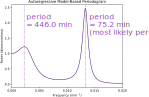
\includegraphics[width=\textwidth]{ar}
   \caption{
   }
   \label{fig:analysis-ar-periodogram}
  \end{subfigure}

  \caption{
    \textbf{(\ref{fig:analysis-ar-timeseries})}
    Sample time series (dark solid line), with a fitted autoregressive model (light solid line) of order 4 computed according to \textcite{jiaFrequencyDomainAnalysis2020}.
    \textbf{(\ref{fig:analysis-ar-periodogram})}
    Periodogram defined based on parameters of the autoregressive model.
    % The presence of a peak of height greater than 1 indicates that the time series is oscillatory.
    % Furthermore, the locations of peaks estimate the period of oscillation in the original time series.
  }
  \label{fig:analysis-ar}
\end{figure}

Fig.\ \ref{fig:analysis-ar} shows that the autoregressive model was able to correctly identify a time series as oscillatory, as evidenced by a peak in the periodogram.
% of height greater than 1.
In addition, the periodogram correctly identifies a period of \SI{75.2}{\minute}.

\begin{table}
  \centering
  % https://tex.stackexchange.com/a/20295
  \begin{tabular}{l|l|c|c|c}
    \multicolumn{2}{c}{}&\multicolumn{2}{c}{Human-defined labels}&\\
    \cline{3-4}
    \multicolumn{2}{c|}{}&Positive&Negative&\multicolumn{1}{c}{Total}\\
    \cline{2-4}
    \multirow{2}{*}{Predicted by AR model}& Positive & 141 & 83 & 224\\
    \cline{2-4}
    & Negative & 124 & 77 & 201\\
    \cline{2-4}
    \multicolumn{1}{c}{} & \multicolumn{1}{c}{Total} & \multicolumn{1}{c}{265} & \multicolumn{1}{c}{160} & \multicolumn{1}{c}{425}\\
  \end{tabular}
  \caption{
    Confusion matrix to evaluate the performance of using the autoregressive model \parencite{jiaFrequencyDomainAnalysis2020} to detect rhythmicity in the \textit{zwf1$\Delta$} dataset.
  }
  \label{tab:analysis-ar-confusion-matrix}
\end{table}

To assess the performance of the use of the autoregressive model for rhythmicity detection across a dataset, I extended this method across the \textit{zwf1$\Delta$} dataset, treating Type I power spectra (Fig.\ \ref{fig:analysis-ar-classification}) as non-oscillatory.
The confusion matrix (table~\ref{tab:analysis-ar-confusion-matrix}) suggests that the method leads to poor accuracy ($a = 0.513$).

% MOVE THIS TO DISCUSSION?
% Furthermore, unlike the classifier based on \textcite{glynnDetectingPeriodicPatterns2006a}, the autoregressive model does not having a parameter that can be adjusted to change the expected proportion of a dataset to be classified as oscillatory --- in other words, the tolerance of detecting rhythmicity cannot be adjusted.
% DISCUSSION
%Alternatively, the order of the model can be treated as a parameter, and model selection can be performed.
%Nevertheless, among the time series that the algorithm classifies as oscillatory, the algorithm accurately estimates the frequency of oscillations.
%[Need: figures to summarise my investigation on population.  Probably need to re-do this on some datasets because it is poorly documented in my notes.]


\subsection{Rhythmicity detection using machine learning}
\label{subsec:analysis-classification-ml}

As an alternative to the mathematical methods previously discussed, I trained a support vector classifier to classify oscillatory and non-oscillatory time series from the \textit{zwf1$\Delta$} cells (appendix \ref{append:analysis-ml}).

% DATA PROCESSING
To pre-process the data, I normalised each time series $x_{i} = x_{i,1}, x_{i,2}, \ldots , x_{i,j}, \ldots x_{i,n}$ to produce a processed time series $z_{i} = z_{i,1}, z_{i,2}, \ldots , z_{i,j}, \ldots z_{i,n}$ as follows:

\begin{equation}
  z_{i,j} = \frac{x_{i,j} - \mu_{i}}{\sigma_{i}}
  \label{eq:analysis-stdscore}
\end{equation}

where $\mu_{i}$ is the mean value of $x_{i}$, and $\sigma_{i}$ is the standard deviation of $x_{i}$.
As a result, each normalised time series $z_{i}$ has a mean of 0 and a standard deviation of 1, therefore ensuring that the dynamic ranges of the fluorescence signals do not affect rhythmicity detection.

% LABELLING
Based on the normalised time series, I labelled them as non-oscillatory ($n_{0}=224$) and oscillatory ($n_{1}=201$).
% SPLITTING
From this input data, 75\% of the time series formed the training set.

% FEATURISATION
% MODELS
\begin{figure}
  \centering
  \includegraphics[width=0.9\textwidth]{svm_feat_compare_edit.pdf}
  \caption[
  ]{
    (Left) Precision and (right) recall from five-fold cross-validation of support vector classifiers trained using different featurisation methods:
    using the time points as features,
    using the power values in the Fourier spectrum as features,
    and using \emph{catch22} features.
    As a control, the oscillatory and non-oscillatory labels were randomly assigned to the time series and the time points were used as features.
  }
  \label{fig:analysis-precision-recall}
\end{figure}

% \begin{figure}
%   \centering
%   \includegraphics[width=0.7\textwidth]{svm_1_edit.pdf}
%   \caption[
%     Precision-recall curve of binary classifier
%   ]{
%     Precision-recall curve of binary classifier, using \textit{catch22} for featurisation and with a support vector classifier architecture (radial bias kernel, $\gamma = 1/22$, $C = 1$).
%   }
%   \label{fig:analysis-svc-pr}
% \end{figure}

To determine the most effective way to featurise the data, I computed the precision and recall of support vector classifiers trained on data featurised using different methods.
% Precision and recall were chosen as evaluation metrics due to the class imbalance
All support vector classifiers were trained using a radial bias kernel, a kernel coefficient $\gamma = 1/N$, where $N$ is the number of features, and a regularisation parameter $C = 10$.
Fig.\ \ref{fig:analysis-precision-recall} suggests that featurisation using \textit{catch22} and the Fourier spectrum gave comparably high performances, as evidenced by high precision and recall, and with a low degree of overfitting, as evidenced by a small variation of both metrics across the rounds of cross-validation.
%To evaluate the performance of the \textit{catch22}-based classifier, Fig. \ref{fig:analysis-svc-pr} shows the precision-recall curve of the classifier, which suggests a good performance.

% ADAPTATION OF SVM: PREDICT PROBABILITIES
\begin{figure}
  \centering
  \begin{subfigure}[htpb]{0.5\textwidth}
   \centering
   \includegraphics[width=\textwidth]{svm_2_edit.pdf}
   \caption{
   }
   \label{fig:analysis-svc-proba-histogram-model}
  \end{subfigure}%
  \begin{subfigure}[htpb]{0.5\textwidth}
   \centering
   \includegraphics[width=\textwidth]{svm_scramble_2_edit.pdf}
   \caption{
   }
   \label{fig:analysis-svc-proba-histogram-scramble}
  \end{subfigure}

  \caption{
    \textbf{(\ref{fig:analysis-svc-proba-histogram-model})}
    Histogram of probabilities of whether a time series in the test data set is classified as oscillatory by the SVC, and as a control,
    \textbf{(\ref{fig:analysis-svc-proba-histogram-scramble})}
    with labels randomly re-assorted to time series.
  }
  \label{fig:analysis-svc-proba-histogram}
\end{figure}


\begin{figure}
  \centering
  \includegraphics[width=0.8\textwidth]{svm_3_edit.pdf}

  \caption{
    Sample test set time series arranged by probability that each is oscillatory, as predicted by the support vector classifier.
  }
  \label{fig:analysis-svc-proba-gallery}
\end{figure}

To predict the probability that each time series is oscillatory, I extended the support vector classifier to predict probabilities, so as to account for uncertainties.
Prediction of probabilities was performed using Platt scaling \parencite{plattProbabilisticOutputsSupport1999}, as implemented by the \texttt{scikit-learn} package for the Python programming language.
Fig.\ \ref{fig:analysis-svc-proba-histogram-model} suggests that the classifier performed well in discriminating between two classes, as evidenced by the U-shaped histogram of probabilities, in contrast to the control (Fig.\ \ref{fig:analysis-svc-proba-histogram-scramble}).
In addition, these probabilities can also serve as a score for the quality of oscillations, as illustrated by Fig.\ \ref{fig:analysis-svc-proba-gallery}.

% MOVE TO DISCUSSION?
%In sum, a simple machine learning architecture is adequate for rhythmicity detection and also offers a probability score for rhythmicity.


%\section[Characterisation]{Characterisation: I have one time series --- what properties does it have?}
\section{Period estimation using the autocorrelation function}
\label{sec:analysis-characterisation}

Characterising features of oscillatory time series is important as it provides a quantitative measure of how yeast metabolic cycles respond to genetic nutrient perturbations.
% The period of an oscillatory time series is the easiest characteristic to compute a fixed number for because it is well-defined.

To show that the autocorrelation function can be used to estimate the period and noise properties of both symmetric and asymmetric oscillations, I adapted the autocorrelation function as used by \textcite{pietschDeterminingGrowthRates2023} (section~\ref{subsec:methods-computational-xcf}).
To calibrate the method, I generated synthetic oscillations --- sinusoids and the FitzHugh-Nagumo oscillator \parencite{fitzhughImpulsesPhysiologicalStates1961} --- to investigate the effect of their properties on the autocorrelation function (section~\ref{subsec:methods-computational-synthetic}).
Subsequently, I applied the autocorrelation function to characterise experimentally-recorded time series.

\subsection{Synthetic data}
\label{subsubsec:analysis-characterisation-synthetic}

\subsubsection{Harmonic oscillator: effect of noise parameters}
\label{subsubsec:analysis-characterisation-acf-sinusoid}

\begin{figure}
  \centering
  \begin{subfigure}[t]{0.6\textwidth}
  \centering
    \includegraphics[width=\linewidth]{sinusoids_outofphase}
    \caption{
    }
    \label{fig:acf-sinusoids-nonoise-ts}
  \end{subfigure}%
  \centering
  \begin{subfigure}[t]{0.4\textwidth}
  \centering
    \includegraphics[width=\linewidth]{sinusoids_outofphase_acf_corrected}
    \caption{
    }
    \label{fig:acf-sinusoids-nonoise-acf}
  \end{subfigure}

  \begin{subfigure}[t]{0.6\textwidth}
  \centering
    \includegraphics[width=\linewidth]{verynoisysinusoids_outofphase}
    \caption{
    }
    \label{fig:acf-sinusoids-gausnoise-ts}
  \end{subfigure}%
  \centering
  \begin{subfigure}[t]{0.4\textwidth}
  \centering
    \includegraphics[width=\linewidth]{verynoisysinusoids_outofphase_acf}
    \caption{
    }
    \label{fig:acf-sinusoids-gausnoise-acf}
  \end{subfigure}

  \begin{subfigure}[t]{0.6\textwidth}
  \centering
    \includegraphics[width=\linewidth]{gillespie_k5_d0p05_mean}
    \caption{
    }
    \label{fig:acf-sinusoids-gillnoise-ts}
  \end{subfigure}%
  \centering
  \begin{subfigure}[t]{0.4\textwidth}
  \centering
    \includegraphics[width=\linewidth]{gillespie_k5_d0p05_acf}
    \caption{
    }
    \label{fig:acf-sinusoids-gillnoise-acf}
  \end{subfigure}

  \caption{
    %Effect of type of noise on the autocorrelation function.
    \textbf{(\ref{fig:acf-sinusoids-nonoise-ts})} Sample sinusoids without noise, and 
    \textbf{(\ref{fig:acf-sinusoids-nonoise-acf})} its autocorrelation function.
    %
    \textbf{(\ref{fig:acf-sinusoids-gausnoise-ts})} Sample sinusoids with Gaussian noise defined by drawing samples from $\mathcal{N}(0,\sigma^{2}=3)$, and 
    \textbf{(\ref{fig:acf-sinusoids-gausnoise-acf})} its autocorrelation function.
    %
    \textbf{(\ref{fig:acf-sinusoids-gillnoise-ts})} Sample sinusoids of with Gillespie noise ($k_{0} = 5$ and $d_{0} = 0.05$), and 
    \textbf{(\ref{fig:acf-sinusoids-gillnoise-acf})} its autocorrelation function.
    Red line is defined by $y = \me^{-2d_{0}T}$, where $T$ represents the lag in units of period of the sinusoids.
    %
    For each case, the frequency of the sinusoids was 0.03, and there were 100 repeats, randomly out-of-phase.
  }
  \label{fig:acf-sinusoids}
\end{figure}

To compare the effect of Gaussian noise and Gillespie noise on the autocorrelation function, I computed the autocorrelation functions from a population of sinusoids with either type of noise added via elementwise sums.

% [Show working -- i.e. the mathematical derivations that make me expect results?]
% [Equations -- clear lines before/after, rather than having them in-line?]

Fig.\ \ref{fig:acf-sinusoids-nonoise-acf} shows that the autocorrelation function computed from a population of out-of-phase sinusoids can be modelled by a cosine with the same period as the sinusoids.%the function $y(T) = cos(2 \pi T)$, where $f$ is the frequency of the sinusoids and $T$ is the lag in units of the periods of the sinusoid.
%This relationship can be confirmed by deriving from the definition of the autocorrelation function used in this chapter (mathematical derivation in appendix ...).
%
Following this, Fig.\ \ref{fig:acf-sinusoids-gausnoise-acf} shows that the addition of Gaussian noise preserved the point $y(0) = 1$, but the amplitude of the cosine that models the autocorrelation function is decreased.
Furthermore, the variation of the autocorrelation function among time series at long lags is increased, as evidenced by the interquartile range, because less data was used to compute the autocorrelation function at longer lags.% (mathematical derivation in appendix ...).

Gillespie noise is based on the birth-death process, and its two parameters control noise parameters (section~\ref{subsec:methods-computational-synthetic}).
Specifically, given a birth rate $k_{0}$ and a death rate $d_{0}$, the noise has a standard deviation of noise amplitude $A = \sqrt{k_{0}/d_{0}}$ and noise timescale $\tau = 1/d_{0}$.
% [Show working -- i.e. the mathematical derivations that make me expect this exponential fit?]
% Though Peter said this `is not trivial'.
Fig.\ \ref{fig:acf-sinusoids-gillnoise-acf} shows that when Gillespie noise was added to the sinusoids, the medium autocorrelation followed the exponential decay function $y = \me^{-2d_{0}T}$, where $T$ represents lag.
In addition, the locations of the peaks of the autocorrelation function were preserved.
The observation thus suggests that the death rate $d_{0}$ parameter of Gillespie noise controlled the shape of the autocorrelation function.


\begin{figure}
  \centering
  \begin{subfigure}[t]{0.6\textwidth}
  \centering
    \includegraphics[width=\linewidth]{gillespie_k5_d0p5_mean.png}
    \caption{
    }
    \label{fig:acf-noisetimescale-highd0-ts}
  \end{subfigure}%
  \begin{subfigure}[t]{0.4\textwidth}
  \centering
    \includegraphics[width=\linewidth]{gillespie_k5_d0p5_acf.png}
    \caption{
    }
    \label{fig:acf-noisetimescale-highd0-acf}
  \end{subfigure}

  \begin{subfigure}[t]{0.6\textwidth}
  \centering
    \includegraphics[width=\linewidth]{gillespie_k5_d0p005_mean.png}
    \caption{
    }
    \label{fig:acf-noisetimescale-lowd0-ts}
  \end{subfigure}%
  \begin{subfigure}[t]{0.4\textwidth}
  \centering
    \includegraphics[width=\linewidth]{gillespie_k5_d0p005_acf.png}
    \caption{
    }
    \label{fig:acf-noisetimescale-lowd0-acf}
  \end{subfigure}

  \caption[
    Effect of death rate of Gillespie noise on the autocorrelation function.
  ]{
    %Effect of death rate ($d_{0}$) of Gillespie noise on the autocorrelation function.
    \textbf{(\ref{fig:acf-noisetimescale-highd0-ts})} Sample sinusoids with Gillespie noise ($k_{0} = 5$ and $d_{0} = 0.5$), and 
    \textbf{(\ref{fig:acf-noisetimescale-highd0-acf})} its autocorrelation function.
    %
    \textbf{(\ref{fig:acf-noisetimescale-lowd0-ts})} Sample sinusoids with Gillespie noise ($k_{0} = 5$ and $d_{0} = 0.005$), and 
    \textbf{(\ref{fig:acf-noisetimescale-lowd0-acf})} its autocorrelation function.
    %
    Red lines are defined by $y = \me^{-2d_{0}T}$, where $T$ represents the lag in units of period of the sinusoids.
    %
    For each case, the frequency of the sinusoids was 0.03, and there were 100 repeats, randomly out-of-phase.
  }
  \label{fig:acf-noisetimescale}
\end{figure}


\begin{figure}
  \centering
  \begin{subfigure}[t]{0.5\textwidth}
  \centering
    \includegraphics[width=\linewidth]{acf_fit_example.png}
    \caption{
    }
    \label{fig:acf-noisetimescale-effect-fit}
  \end{subfigure}%
  \begin{subfigure}[t]{0.5\textwidth}
  \centering
    \includegraphics[width=\linewidth]{deathrate_vs_decay.png}
    \caption{
    }
    \label{fig:acf-noisetimescale-effect-relationship}
  \end{subfigure}

  \caption{
    %Characterising the autocorrelation function to quantify the effect of Gillespie noise timescale.
    \textbf{(\ref{fig:acf-noisetimescale-effect-fit})} Fitting exponential decay functions to estimate $d_{0}$ from the autocorrelation function.
    \textbf{(\ref{fig:acf-noisetimescale-effect-relationship})} The relationship between $d_{0}$ and the decay rate $D$ found from fitting exponential decay functions to the mean autocorrelation function, the peaks, and the troughs of this mean function.
    Here, $k_{0}$ was held constant at 5.
  }
  \label{fig:acf-noisetimescale-effect}
\end{figure}

To quantify the effect of the noise timescale on the shape of the autocorrelation function, I varied the death rate parameter $d_{0}$ when generating Gillespie noise.
%
Fig.\ \ref{fig:acf-noisetimescale} shows that a higher death rate decreased the decay timescale of the autocorrelation function (Fig.\ \ref{fig:acf-noisetimescale-highd0-ts}), while a lower death rate introduced long-term trends in the simulated signals (Fig.\ \ref{fig:acf-noisetimescale-lowd0-ts}).
A lower death rate also increased the variation between autocorrelation functions between replicates (Fig.\ \ref{fig:acf-noisetimescale-lowd0-acf}).

To show how $d_{0}$ can be estimated from the autocorrelation function, I fit exponential decay functions of the form $y = (1-C)\me^{-DT}+C$ to the mean autocorrelation, the peaks of the mean function, and the troughs of the mean functions using non-linear least squares fitting, defining $C$ and $D$ as variable parameters (Fig.\ \ref{fig:acf-noisetimescale-effect-fit}).
Subsequently, Fig.\ \ref{fig:acf-noisetimescale-effect-relationship} suggests that the decay rates $D$ of the autocorrelation function indeed increases linearly with $d_{0}$.
In other words, the death rate $d_{0}$ controls the decay rate $D$ of the autocorrelation function.
Conversely, if $D$ can be estimated from the autocorrelation function, then the noise timescale of the time series can be estimated.


\begin{figure}
  \centering
  \begin{subfigure}[t]{0.6\textwidth}
  \centering
    \includegraphics[width=\linewidth]{gillespie_k25_d0p05_mean.png}
    \caption{
    }
    \label{fig:acf-noiseamplitude-highk0-ts}
  \end{subfigure}%
  \begin{subfigure}[t]{0.4\textwidth}
  \centering
    \includegraphics[width=\linewidth]{gillespie_k25_d0p05_acf.png}
    \caption{
    }
    \label{fig:acf-noiseamplitude-highk0-acf}
  \end{subfigure}

  \begin{subfigure}[t]{0.6\textwidth}
  \centering
    \includegraphics[width=\linewidth]{gillespie_k1_d0p05_mean.png}
    \caption{
    }
    \label{fig:acf-noiseamplitude-lowk0-ts}
  \end{subfigure}%
  \begin{subfigure}[t]{0.4\textwidth}
  \centering
    \includegraphics[width=\linewidth]{gillespie_k1_d0p05_acf.png}
    \caption{
    }
    \label{fig:acf-noiseamplitude-lowk0-acf}
  \end{subfigure}

  \caption[
    Effect of birth rate of Gillespie noise on the autocorrelation function.
  ]{
    %Effect of birth rate ($k_{0}$) of Gillespie noise on the autocorrelation function.
    \textbf{(\ref{fig:acf-noiseamplitude-highk0-ts})} Sample sinusoids with Gillespie noise ($k_{0} = 25$ and $d_{0} = 0.05$), and 
    \textbf{(\ref{fig:acf-noiseamplitude-highk0-acf})} its autocorrelation function.
    %
    \textbf{(\ref{fig:acf-noiseamplitude-lowk0-ts})} Sample sinusoids with Gillespie noise ($k_{0} = 1$ and $d_{0} = 0.05$), and 
    \textbf{(\ref{fig:acf-noiseamplitude-lowk0-acf})} its autocorrelation function.
    %
    Red lines are defined by $y = \me^{-2d_{0}T}$, where $T$ represents the lag in units of period of the sinusoids.
    %
    For each case, the frequency of the sinusoids was 0.03, and there were 100 repeats, randomly out-of-phase.
  }
  \label{fig:acf-noiseamplitude}
\end{figure}


\begin{figure}
  \centering
  \includegraphics[width=0.6\linewidth]{birthrate_vs_ydispl.png}
  \caption[
    Quantifying the effect of Gillespie noise amplitude on the autocorrelation function
  ]{
    The relationship between the noise amplitude and the $y$-displacement $C$ found from fitting exponential decay functions to the mean autocorrelation function, the peaks, and the troughs of this mean function.
    Here, $d_{0}$ was held constant at 0.05.
  }
  \label{fig:acf-noiseamplitude-effect}
\end{figure}


To quantify the effect of the noise amplitude, I varied the birth rate parameter $k_{0}$ when generating Gillespie noise (Fig.\ \ref{fig:acf-noiseamplitude}).
%
Fig.\ \ref{fig:acf-noiseamplitude} shows that a lower birth rate decreased the amplitude of noise (Fig.\ \ref{fig:acf-noiseamplitude-lowk0-ts}) and decreased the variation between replicate autocorrelation functions (Fig.\ \ref{fig:acf-noiseamplitude-lowk0-acf}), while the opposite was true for a higher birth rate (Figs.\ \ref{fig:acf-noiseamplitude-highk0-ts}--\ref{fig:acf-noiseamplitude-highk0-acf}).

To show how the noise amplitude can be estimated from the autocorrelation function, I fit exponential decay functions as in Fig.\ \ref{fig:acf-noisetimescale-effect-fit}.
Fig.\ \ref{fig:acf-noiseamplitude-effect} suggests that the $y$-displacements $C$ of the exponential fits to peaks and troughs converged to 0 as $k_{0}/d_{0}$ increased, showing that the amplitude of the oscillations in the autocorrelation function decreases as the noise amplitude increases.
In other words, the birth rate $d_{0}$ controls the $y$-displacement parameter $C$ of the autocorrelation function, which is a proxy for the function's amplitude.
Conversely, if $C$ can be estimated from the autocorrelation function, then the noise amplitude of the time series can be estimated.

% [Move to conclusion?]
% To conclude, if a population of replicate oscillatory time series is modelled with the sum of sinusoids and Gillespie noise, then the birth rate and death rate can control the shape of the autocorrelation function.
% The death rate controls the timescale of noise and thus how fast the autocorrelation decays as lag increases.
% The birth rate controls the amplitude of noise and thus controls how robust the autocorrelation function is.


\subsubsection{FitzHugh-Nagumo oscillator: effect of oscillator shape}
\label{subsubsec:analysis-characterisation-acf-fhn}


\begin{figure}
  \centering
  \begin{subfigure}[t]{0.6\textwidth}
  \centering
    \includegraphics[width=\linewidth]{fhn_meanplot}
    \caption{
    }
    \label{fig:acf-fhn-gillnoise-ts}
  \end{subfigure}%
  \begin{subfigure}[t]{0.4\textwidth}
  \centering
    \includegraphics[width=\linewidth]{fhn_acf}
    \caption{
    }
    \label{fig:acf-fhn-gillnoise-acf}
  \end{subfigure}

  \caption{
    %The autocorrelation function of FitzHugh-Nagumo oscillators with Gillespie noise.
    \textbf{(\ref{fig:acf-fhn-gillnoise-ts})} Sample FitzHugh-Nagumo oscillators ($RI_{\mathrm{ext}}$ = 0.4, $\tau$ = 12.5, $a$ = 0.7, $b$ = 0.82) with Gillespie noise ($k_{0} = 5$ and $d_{0} = 0.05$), and 
    \textbf{(\ref{fig:acf-fhn-gillnoise-acf})} its autocorrelation function.
    Red line is defined by $y = \me^{-2d_{0}T}$, where $T$ represents the lag in units of period of the sinusoids.
    %
    There were 100 repeats, randomly out-of-phase.
  }
  \label{fig:acf-fhn}
\end{figure}


\begin{figure}
  \centering
  \begin{subfigure}[t]{0.45\textwidth}
  \centering
    \includegraphics[width=\linewidth]{fhn_expofit}
    \caption{
    }
    \label{fig:acf-fhn-noiseparams-fit}
  \end{subfigure}%
  \begin{subfigure}[t]{0.45\textwidth}
  \centering
    \includegraphics[width=\linewidth]{fhn_highnts_expofit}
    \caption{
    }
    \label{fig:acf-fhn-noiseparams-fit-highnts}
  \end{subfigure}

  \begin{subfigure}[t]{0.45\textwidth}
  \centering
    \includegraphics[width=\linewidth]{fhn_deathrate_vs_decay.png}
    \caption{
    }
    \label{fig:acf-fhn-noiseparams-noisetimescale}
  \end{subfigure}%
  \begin{subfigure}[t]{0.45\textwidth}
  \centering
    \includegraphics[width=\linewidth]{fhn_birthrate_vs_ydispl.png}
    \caption{
    }
    \label{fig:acf-fhn-noiseparams-noiseamplitude}
  \end{subfigure}

  \caption{
    %Quantifying the effect of Gillespie noise parameters on the autocorrelation function of FitzHugh-Nagumo oscillators.
    \textbf{(\ref{fig:acf-fhn-noiseparams-fit})}
    Fitting exponential decay functions of the form $y = (1-C)\me^{-DT}+C$, with $C$ and $D$ as variable parameters, to the autocorrelation function, generated with $k_{0}=5$ and $d_{0}=0.05$, and
    \textbf{(\ref{fig:acf-fhn-noiseparams-fit-highnts})}
    with $k_{0}=5$ and $d_{0}=0.005$.
    \textbf{(\ref{fig:acf-fhn-noiseparams-noisetimescale})}
    The relationship between $d_{0}$ and the decay rate $D$ ($k_{0}=5$).
    \textbf{(\ref{fig:acf-fhn-noiseparams-noiseamplitude})}
    The relationship between $k_{0}/d_{0}$ and $y$-displacement $C$ of the exponential fit ($d_{0}=0.05$)
  }
  \label{fig:acf-fhn-noiseparams}
\end{figure}

To test whether Gillespie noise parameters can be estimated from the autocorrelation function computed from oscillations of a different shape, I repeated the exponential fitting in section~\ref{subsubsec:analysis-characterisation-acf-sinusoid} on the FitzHugh-Nagumo oscillator.

Fig.\ \ref{fig:acf-fhn-gillnoise-acf} shows that when the oscillator had a different shape, the shape of the autocorrelation function changed: i.e.\ the waves in the autocorrelation function were more pointed.
In addition, fitting an exponential decay function to the autocorrelation function to estimate noise parameters was less reliable, particularly with high noise timescales (Fig.\ \ref{fig:acf-fhn-noiseparams-fit-highnts}).
As a consequence, estimating the noise timescale $\tau$ from the decay rate $D$ of the exponential decay function produced a greater range of uncertainty (Fig.\ \ref{fig:acf-fhn-noiseparams-noisetimescale}).
However, estimating the noise amplitude $A$ based on the y-displacement $C$ of the exponential decay function remained as reliable as the sinusoid oscillator case (Fig.\ \ref{fig:acf-fhn-noiseparams-noiseamplitude}).


\subsection{Real data}
\label{subsubsec:analysis-characterisation-real}

\begin{figure}
  \centering
  \begin{subfigure}[t]{0.8\textwidth}
  \centering
    \includegraphics[width=\linewidth]{acf_sinusoid_biol_ts.png}
    \caption{
    }
    \label{fig:acf-sinusoid-biol-ts}
  \end{subfigure}

  \begin{subfigure}[t]{0.5\textwidth}
  \centering
    \includegraphics[width=\linewidth]{acf_sinusoid_biol_acf.png}
    \caption{
    }
    \label{fig:acf-sinusoid-biol-acf}
  \end{subfigure}%
  \begin{subfigure}[t]{0.5\textwidth}
  \centering
    \includegraphics[width=\linewidth]{acf_sinusoid_biol_acf_fit.png}
    \caption{
    }
    \label{fig:acf-sinusoid-biol-acf-fit}
  \end{subfigure}

  \caption{
    \textbf{(\ref{fig:acf-sinusoid-biol-ts})}
    Sample time series of flavin autofluorescence.
    \textbf{(\ref{fig:acf-sinusoid-biol-acf})}
    Autocorrelation function across a population of time series of flavin autofluorescence.
    \textbf{(\ref{fig:acf-sinusoid-biol-acf})}
    Fitting exponential decay functions to determine noise parameters, lag axis scaled to match Fig.\ \ref{fig:acf-noisetimescale-effect}.
  }
  \label{fig:acf-sinusoid-biol}
\end{figure}

To deduce the period and noise parameters of a experimentally-recorded sinusoid-like signal (Fig.\ \ref{fig:acf-sinusoid-biol-ts}), I computed the autocorrelation functions of a population of flavin autofluorescence time series (Fig.\ \ref{fig:acf-sinusoid-biol-acf}), and fitted exponential functions to the mean autocorrelation function (Fig.\ \ref{fig:acf-sinusoid-biol-acf-fit}).
The autocorrelation function suggests an average period of 19 time points, corresponding to \SI{95}{\minute}, as expected from the environmental conditions.
However, estimation of noise parameters was complicated by the damping in the autocorrelation function, giving a different shape compared to the synthetic data and fewer peaks and troughs for fitting.
Nevertheless, the decay rate $D$ of the exponential function fitted to the mean autocorrelation function suggested a noise timescale of 7.16 and the y-displacement $C$ of the exponential function fitted to the peaks of the autocorrelation function suggested a noise amplitude of 161.84.


\begin{figure}
  \centering
  \begin{subfigure}[t]{0.8\textwidth}
  \centering
    \includegraphics[width=\linewidth]{acf_fhn_biol_ts.png}
    \caption{
    }
    \label{fig:acf-fhn-biol-ts}
  \end{subfigure}

  \begin{subfigure}[t]{0.5\textwidth}
  \centering
    \includegraphics[width=\linewidth]{acf_fhn_biol_acf.png}
    \caption{
    }
    \label{fig:acf-fhn-biol-acf}
  \end{subfigure}%
  \begin{subfigure}[t]{0.5\textwidth}
  \centering
    \includegraphics[width=\linewidth]{acf_fhn_biol_acf_fit.png}
    \caption{
    }
    \label{fig:acf-fhn-biol-acf-fit}
  \end{subfigure}

  \caption{
    \textbf{(\ref{fig:acf-fhn-biol-ts})}
    Sample time series of histone 2B abundance.
    \textbf{(\ref{fig:acf-fhn-biol-acf})}
    Autocorrelation function across a population of time series of histone 2B abundance.
    \textbf{(\ref{fig:acf-fhn-biol-acf})}
    Fitting exponential decay functions to determine noise parameters.
  }
  \label{fig:acf-fhn-biol}
\end{figure}

Similarly, to deduce the period and noise parameters of a experimentally-recorded asymmetric signal (Fig.\ \ref{fig:acf-fhn-biol-ts}), I computed the autocorrelation functions of a population of histone 2B abundance time series (Fig.\ \ref{fig:acf-fhn-biol-acf}), and fitted exponential functions to the mean autocorrelation function (Fig.\ \ref{fig:acf-fhn-biol-acf-fit}).
The autocorrelation function also suggests an average period of 19 time points, corresponding to \SI{95}{\minute}.
As was the case for the flavin autofluorescence time series, the damping in the autocorrelation function complicated estimation of noise parameters; though the decay rate $D$ of the exponential function fitted to the mean autocorrelation function suggested a noise timescale of 11.19 and the y-displacement $C$ of the exponential function fitted to the peaks of the autocorrelation function suggested a noise amplitude of 292.41.
The differences of these noise parameters relative to the flavin autofluorescence time series suggest different noise properties, which can be explained by the different fluorescence channels and exposure times used to generate each type of signal.

%\section[Correlation]{Correlation: I have two signals from the same cell --- what are their relationships to each other?}
\section{Detection of synchrony}
\label{sec:analysis-correlation}

To test a method to quantify the temporal lag between two types of oscillations, I computed the cross-correlation functions of a population of sinusoid and FitzHugh-Nagumo oscillators.
Cross-correlation has been used to investigate the relationship between the expression levels of two genes in a model feed-forward loop \parencite{dunlopRegulatoryActivityRevealed2008},
and to investigate the relationship between instantaneous growth rate and the expression of \textit{lac} genes of enzymes in central metabolism across a population of \textit{E. coli} cells \parencite{kivietStochasticityMetabolismGrowth2014}.
%Importantly, \textcite{kivietStochasticityMetabolismGrowth2014} employed a single-cell microfluidics experiment with time-lapse microscopy, and therefore their analysis of a population of time series is applicable in this chapter.

\subsection{Synthetic data}
\label{subsubsec:analysis-correlation-synthetic}

\begin{figure}
  \centering
  \begin{subfigure}[t]{0.6\textwidth}
  \centering
    \includegraphics[width=\linewidth]{sinusoid_and_fitzhughnagumo_nonoise.png}
    \caption{
    }
    \label{fig:xcf-nonoise-ts}
  \end{subfigure}%
  \centering
  \begin{subfigure}[t]{0.4\textwidth}
  \centering
    \includegraphics[width=\linewidth]{randomshift_sinusoid_fitzhughnagumo_xcf.png}
    \caption{
    }
    \label{fig:xcf-nonoise-xcf}
  \end{subfigure}

  \begin{subfigure}[t]{0.6\textwidth}
  \centering
    \includegraphics[width=\linewidth]{sinusoid_and_fitzhughnagumo_gillnoise.png}
    \caption{
    }
    \label{fig:xcf-gillnoise-ts}
  \end{subfigure}%
  \centering
  \begin{subfigure}[t]{0.4\textwidth}
  \centering
    \includegraphics[width=\linewidth]{randomshift_sinusoid_fitzhughnagumo_gillnoise_xcf.png}
    \caption{
    }
    \label{fig:xcf-gillnoise-xcf}
  \end{subfigure}

  \caption{
    %Using the cross-correlation function to evaluate the shift of one synthetic time series relative to another with a different shape.
    \textbf{(\ref{fig:xcf-nonoise-ts})}
    (Blue) Sample sinusoid ($f = 0.0235$) and (orange) FitzHugh-Nagumo oscillator ($RI_{\mathrm{ext}}$ = 0.4, $\tau$ = 12.5, $a$ = 0.7, $b$ = 0.82) of the same frequency and without noise, and
    \textbf{(\ref{fig:xcf-nonoise-xcf})}
    the cross-correlation function of the FitzHugh-Nagumo oscillators with respect to the sinusoids.
    %
    \textbf{(\ref{fig:xcf-gillnoise-ts})}
    (Blue) Sample sinusoid and (orange) FitzHugh-Nagumo oscillator with same parameters as \ref{fig:xcf-nonoise-ts}, but with Gillespie noise ($d_{0} = 0.05$, $k_{0} = 5$), and
    \textbf{(\ref{fig:xcf-gillnoise-xcf})}
    the cross-correlation function of the FitzHugh-Nagumo oscillators with respect to the sinusoids.
    %
    For each case, there were 400 repeats, randomly out-of-phase.
  }
  \label{fig:xcf}
\end{figure}

Fig.\ \ref{fig:xcf-nonoise-xcf} shows that the cross-correlation function identifies that the sinusoids, on average, peak 20 time points before the FitzHugh-Nagumo oscillators, close to the actual value of 20.75 time points.
This shift was evidenced by the position of the peak of the cross-correlation function closest to the vertical axis.
The cross-correlation function further shows that synchrony between the two oscillators is maintained along the entire time series, across all time series.
Furthermore, Fig.\ \ref{fig:xcf-gillnoise-xcf} suggests that even with strong Gillespie noise, the lag between the two oscillators could still be deduced from the cross-correlation function.


\subsection{Real data}
\label{subsubsec:analysis-correlation-real}


\begin{figure}
  \centering
  \begin{subfigure}[t]{1.0\textwidth}
  \centering
    \includegraphics[width=\linewidth]{single_birth_plot_nostar.pdf}
    \caption{
    }
    \label{fig:xcf-biol-ts}
  \end{subfigure}

  \begin{subfigure}[t]{0.7\textwidth}
  \centering
    \includegraphics[width=\linewidth]{xcf_edit.pdf}
    \caption{
    }
    \label{fig:xcf-biol-xcf}
  \end{subfigure}

  \caption{
    \textbf{(\ref{fig:xcf-biol-ts})}
    Sample time series of flavin autofluorescence (blue) and histone 2B abundance (orange).
    \textbf{(\ref{fig:xcf-biol-xcf})}
    Cross-correlation function between the flavin autofluorescence time series and the histone 2B abundance time series.
  }
  \label{fig:xcf-biol}
\end{figure}

To show how the cross-correlation function can be used to quantify the synchrony between flavin autofluorescence oscillations and HTB2::mCherry levels in a population of cells, Fig.\ \ref{fig:xcf-biol} displays a sample pair of time series (Fig.\ \ref{fig:xcf-biol-ts}) and the cross-correlation function from the population of cells (Fig.\ \ref{fig:xcf-biol-xcf}).
The cross-correlation function suggests that the histone 2B oscillations peaked after the flavin autofluorescence oscillations by an average of \SI{5}{\minute}.


\section{Discussion}
\label{sec:analysis-discussion}

This chapter discusses methods to filter long-term trends in time series data, to visualise structures within a dataset of time series, to detect rhythmicity in a time series, to estimate period and noise parameters, and to detect the synchrony between two time series.

My results suggest that using a high-pass Butterworth filter to filter out long-term trends in time series data gives better control over the frequency profile of the time series than moving-average methods, which is often used to detrend time series from biological oscillators.
Such results highlight that a degree of caution is needed to choose methods for a crucial step in data analysis.

My exploration of UMAP and modularity clustering suggests that both methods are useful to discovering structure within time series, particularly along the division between oscillatory and non-oscillatory time series.
These methods further indicate sub-groups of time series that may have similar properties, such as shape or oscillation quality, which may correspond to sub-populations of metabolic cycle-producing cells in a culture.
The consistency between the two methods strongly suggest that such groups in the dataset are meaningful.

Subsequently, my exploration of three approaches to detect rhythmicity --- deriving a statistical test of a power spectrum, deriving a periodogram from an autoregressive model, and a support vector classifier --- highlights the difficulty of rhythmicity detection in noisy biological time series.
The spectral method described by \parencite{glynnDetectingPeriodicPatterns2006a} had a modest performance, but required defining a threshold and was dependent the input dataset.
The autoregressive model was able to identify the most likely period in some time series, but otherwise classifies most time series as non-oscillatory, and lacks a tuning parameter.
Finally, the support vector classifier suggests that a simple machine learning model can be adapted for rhythmicity detection, subject to a good feature set and training data.
Ultimately, rhythmicity detection requires supplying a threshold in some form, be it a range of frequencies in which oscillations are expected, a parameter that controls the proportion of time series detected as oscillatory, or training labels.

My observations concerning the autocorrelation function confirms its use for estimating the period of an oscillatory time series, as used previously by \parencite{papagiannakisAutonomousMetabolicOscillations2017}.
As periodicity-estimation methods have a limited ability to estimate the period of short, noisy time series owing to little input data, it can be useful to combine several such methods to produce a picture of the periodicity of oscillatory time series; for example, \textcite{potvin-trottierSynchronousLongtermOscillations2016} combines the autocorrelation function and the Fourier transform to study the changes in the periodicity of a modified model of the repressilator.
Furthermore, I showed that the autocorrelation function may be used to estimate parameters to describe noise, assuming that the noise can be modelled by the birth-death process.
However, further work, such as synthetic time series generated from a wider variety of parameters or additional estimation methods are likely required for adequate estimation of noise parameters from real data.
In addition, it is possible that other types of noise better describe the noise from real data, and such types of noise may lead to different effects on the autocorrelation function.

Finally, my results show that the cross-correlation function, as used by \textcite{dunlopRegulatoryActivityRevealed2008}, \textcite{kivietStochasticityMetabolismGrowth2014}, and \textcite{pietschDeterminingGrowthRates2023}, can be used to detect synchrony between two sets of time series and to quantify the temporal relationship between the time series, even if the time series are very noisy.

Taken together, the analysis methods discussed in this chapter can form the basis of a powerful data analysis pipeline to analyse large datasets of potentially oscillatory biological time series.

\chapter{Microfluidics and fluorescence microscopy for cellular metabolic cycles}
\label{ch:biology}

To reconcile the evidence about the characteristics of the YMC from single-cell and chemostat experiments, I sought to use a single-cell experimental platform to address whether cellular metabolic cycles confirm chemostat-based studies.

There is a paucity of studies of the yeast metabolic cycle at the cellular level --- i.e.\ in which budding yeast cells are investigated in isolation rather than as a population.
Previous population-level studies in the chemostat, by their very nature, fail to account for cell-to-cell heterogeneity and create cell density and environmental conditions that are far removed from the natural habitat of budding yeast.

Here, I use single-cell microfluidics to physically separate budding yeast cells and use fluorescence microscopy to monitor the yeast metabolic cycle and the cell division cycle.

Specifically, I aim to evaluate these hypotheses:
\begin{enumerate}
  \item Yeast cells independently generate yeast metabolic cycles.
        Each cell generates the metabolic cycle autonomously of other cellular oscillators and itself can phase-lock the cell division cycle.
  \item The yeast metabolic cycle is retained in different nutrient and genetic perturbations, but characteristics of the oscillator change as an adaptation response.
  \item Flavin autofluorescence read-outs of the yeast metabolic cycle in single cells recapitulate oscillations in dissolved oxygen from the yeast metabolic cycle in the chemostat.
        If there are discrepancies between the two manifestations of the yeast metabolic cycle, cell-to-cell heterogeneity should explain them.
\end{enumerate}

In this chapter, I showed that metabolic cycles are generated autonomously and are coupled to the cell division cycle in permissive conditions, confirming previous single-cell studies.
To induce decoupling between the two oscillators, confirming the independence and autonomy of the metabolic oscillator, I used fast nutrient switching to induce starvation.
I further showed that the metabolic cycle was robust and adapted to nutrient and genetic perturbations.
Finally, to address whether single-cell metabolic cycles confirm findings from chemostat-based experimental studies, I emulated situations known to affect dissolved-oxygen traces: potassium deficiency, and deletions of genes with roles in metabolic and biological timekeeping.


\section[Permissive conditions]{Single-cell flavin oscillations synchronise with cell division cycle in permissive conditions.}
\label{sec:biology-sync}

\begin{figure}
  \centering
    \includegraphics[width=0.5\linewidth]{garmendia-torresMultipleInputsEnsure2018_1_adapted.jpg}
    \caption{
      Engineering a fluorescent protein cassette fused to \textit{HTB2} (A) allows the identification of phases of the cell division cycle by modelling the fluorescent protein intensity changes over time as piecewise linear sections (B).
      Adapted from \textcite{garmendia-torresMultipleInputsEnsure2018}.
    }
  \label{fig:biology-htb2}
\end{figure}

To show that metabolic cycles are generated autonomously and are coupled to the cell division cycle, I replicated the single-cell flavin oscillations observed by \textcite{baumgartnerFlavinbasedMetabolicCycles2018} that supported these observations.
Replicating results from a previous flavin-based microfluidics study is important to confirm that the microfluidics set-up I used truly monitored the yeast metabolic cycle, especially if the set-up differed from previous studies \parencite{papagiannakisAutonomousMetabolicOscillations2017, baumgartnerFlavinbasedMetabolicCycles2018}.

Fig.\ \ref{fig:biology-highglc-single} shows that oscillations in flavin fluorescence peak when a bud forms in GS/M, as evidenced by prototrophic FY4 HTB2::mCherry cells grown in minimal medium supplemented with \SI{20}{\gram~\litre^{-1}} glucose.
The HTB2::mCherry insertion allows monitoring phases of the cell division cycle via imaging and quantifying the intensity of the inserted fluorescent protein \parencite{garmendia-torresMultipleInputsEnsure2018}, while also allowing monitoring flavin fluorescence by avoiding overlap of emission spectra.

As observed, oxidation of flavin upon budding was expected for these reasons:
\begin{enumerate}
  \item Flavin fluorescence peaks (oxidised form) and NAD(P)H fluorescence peaks (reduced form) at the same time in chemostat cultures \parencite{murrayRedoxRegulationRespiring2011}.
  \item NAD(P)H is in the reduced form when buds form \parencite{papagiannakisAutonomousMetabolicOscillations2017}.
  \item The flavoprotein lipoamide dehydrogenase is in redox equilibrium with NAD(P)H \parencite{sianoNADHFlavinFluorescence1989}.
\end{enumerate}

\begin{figure}
  \centering
    \includegraphics[width=1.0\linewidth]{single_birth_plot_edit.pdf}
    \caption{
      Oscillations of flavin fluorescence in the yeast metabolic cycle synchronise with events in the cell division cycle.
      Figure shows sample flavin fluorescence (purple, solid lines) and histone 2B (pink, dotted lines) level in a single FY4 HTB2::mCherry cell grown in \SI{20}{\gram~\litre^{-1}} glucose.
      Vertical lines (black, dashed) indicate budding.
    }
  \label{fig:biology-highglc-single}
\end{figure}

Fig.\ \ref{biology-highglc-single} also shows that in some cases, a metabolic oscillation occurred without cell division cycle progression or bud formation.
Such cases, also revealed by \textcite{papagiannakisAutonomousMetabolicOscillations2017} via NAD(P)H cycles, confirmed that the metabolic cycle is generated autonomously from the cell division cycle.


\begin{figure}
  \centering
  \begin{subfigure}[htpb]{0.4\textwidth}
   \centering
   \includegraphics[width=\textwidth]{htb2mCherry_26643_14}
   \caption{
    Mean Fourier spectrum of flavin fluorescence across cells.
   }
   \label{fig:biology-highglc-sync-fourier}
  \end{subfigure}%
  \begin{subfigure}[htpb]{0.4\textwidth}
   \centering
   \includegraphics[width=\textwidth]{htb2mCherry_26643_12}
   \caption{
     \textbf{(Main)} Median autocorrelation functions of flavin fluorescence (blue) and histone 2B levels (orange) time series,
     along with \textbf{(inset)} the periods of each oscillator across cells as determined by the strongest frequency in each signal's Fourier spectrum.
   }
   \label{fig:biology-highglc-sync-acf}
  \end{subfigure}

  \caption{
    Insert caption here.
  }
  \label{fig:biology-highglc-sync-spectral}
\end{figure}

\begin{figure}
  \centering
  \begin{subfigure}[htpb]{0.4\textwidth}
   \centering
   \includegraphics[width=\textwidth]{heatmap_edit.pdf}
   \caption{
     Heatmap shows the flavin fluorescence (pixels on a red-blue scale) and budding events (black pixels) of each cell.
     Signals are aligned by the first budding event.
   }
   \label{fig:biology-highglc-sync-heatmap}
  \end{subfigure}%
  \begin{subfigure}[htpb]{0.4\textwidth}
   \centering
   \includegraphics[width=\textwidth]{htb2mCherry_26643_6}
   \caption{
    Median flavin fluorescence signal across cells, aligned to first budding event.
   }
   \label{fig:biology-highglc-sync-median}
  \end{subfigure}

  \begin{subfigure}[htpb]{0.4\textwidth}
   \centering
   \includegraphics[width=\textwidth]{xcf_edit.pdf}
   \caption{
    Cross-correlation between flavin and histone 2B signals.
   }
   \label{fig:biology-highglc-sync-xcf}
  \end{subfigure}

  \caption{
    The yeast metabolic cycle and cell division cycle synchronise within each cell in a population of FY4 HTB2::mCherry cells under the same conditions (\SI{20}{\gram~\litre^{-1}} glucose).
  }
  \label{fig:biology-highglc-sync-corr}
\end{figure}

To quantify the period of the oscillators, I used several time series analysis methods in concert.
Fig.\ \ref{fig:biology-highglc-sync-spectral} shows that the mean Fourier spectrum and median autocorrelation function both suggest that flavin fluorescence oscillated at a period of $\approx$\SI{90}{\minute}.
Fig.\ \ref{fig:biology-highglc-sync-acf} additionally shows that the cell division cycle proceeds at the same frequency, as evidenced by the autocorrelation function of mCherry.
This periodicity agrees with the literature regarding the duration of the cell division cycle in such permissive growth conditions. % [CITATIONS NEEDED]

% <text> Move this to fig caption(s)
% In figure~\ref{fig:biology-highglc-sync-heatmap},
% each row of pixels represents a cell.
% Fluorescence is represented as colours (red-blue), with red indicating low signal and blue indicating high signal.
% Each budding event is indicated as a black pixel.
% Signals are aligned by the first budding event to show that
% </text>
To visualise the relationship between the metabolic cycle and the cell division cycle,
Fig.\ \ref{fig:biology-highglc-sync-corr} shows that
(a) budding events synchronise with peaks in fluorescence, and
(b) the cell division cycle varies between cells,
but most are just under \SI{2}{\hour}, agreeing with Fig.\ \ref{fig:biology-highglc-sync-acf} (inset).
The oscillatory shape of the median (Fig.\ \ref{fig:biology-highglc-sync-median}) further confirms the synchrony between the metabolic cycle and budding events.

Finally, to quantify the relationship between the metabolic cycle and the cell division cycle, I computed the cross-correlation function between the flavin and mCherry signals across the population (figure~\ref{fig:biology-highglc-sync-xcf}).
This function shows that the mCherry signals are, on average, shifted by \SI{5}{\minute} relative to the flavin signals.


\section[Abrupt nutrient changes]{Cells autonomously generate flavin oscillations, independently of the cell division cycle, in response to abrupt nutrient changes.}
\label{sec:biology-abrupt}

To provide additional evidence that cells generate metabolic oscillations independent of the cell division cycle, I created a condition in which cells do not undergo cell division.
Specifically, I did so by inducing starvation: I cultured FY4 and HTB2::mCherry cells in \SI{7.5}{\gram~\litre^{-1}} glucose for \SI{7}{\hour} before being abruptly switched to \SI{0}{\gram~\litre^{-1}} glucose for \SI{8}{\hour} and then resumed to \SI{7.5}{\gram~\litre^{-1}} glucose for \SI{7}{\hour} (figure~\ref{fig:biology-starvation}).
This abrupt induction of starvation is similar to experiments described by \textcite{bagameryPutativeBetHedgingStrategy2020} that showed the heterogeneity of cellular responses to starvation.

\begin{figure}
  \centering
  \begin{subfigure}[htpb]{1.0\textwidth}
   \centering
   \includegraphics[width=\textwidth]{starvation_single_birth_plot_new_edit.pdf}
   \caption{
     Flavin fluorescence synchronises with the cell division cycle in high-glucose conditions before and after starvation (FY4 HTB2::mCherry).
     %Figure shows sample flavin fluorescence levels (purple) and histone 2B localisation (pink) in single cells.
     %Vertical lines (black) indicate budding.
   }
   \label{fig:biology-starvation-single}
  \end{subfigure}

  \begin{subfigure}[htpb]{0.7\textwidth}
   \centering
   \includegraphics[width=\textwidth]{heatmap_012_edit.pdf}
   \caption{
     Heatmap shows the flavin fluorescence of each cell (FY4) in a population over time.
     %Each row of pixels represents one of 60 cells.
     %Fluorescence is represented as colours with blue indicating low signal and red indicating high signal.
     Each budding event is indicated as a black pixel.
     During starvation, synchronisation of flavin oscillations between cells were observed, and budding events were sparse.
   }
   \label{fig:biology-starvation-heatmap}
  \end{subfigure}

  \caption{
     Metabolic cycles between physically separated cells synchronise upon abrupt starvation.
     FY4 and HTB2::mCherry cells were grown in \SI{7.5}{\gram~\litre^{-1}} glucose for \SI{7}{\hour} before being abruptly switched to \SI{0}{\gram~\litre^{-1}} glucose for \SI{8}{\hour} and then resumed to \SI{7.5}{\gram~\litre^{-1}} glucose for \SI{7}{\hour}.
  }
  \label{fig:biology-starvation}
\end{figure}


\begin{figure}
  \centering
  \begin{subfigure}[htpb]{0.7\textwidth}
   \centering
   \includegraphics[width=\textwidth]{allstrains_19972_gr}
   \caption{
     Growth rate
   }
   \label{fig:biology-starvation-gr}
  \end{subfigure}

  \begin{subfigure}[htpb]{0.7\textwidth}
   \centering
   \includegraphics[width=\textwidth]{allstrains_19972_budprob}
   \caption{
     Budding probability
   }
   \label{fig:biology-starvation-budprob}
  \end{subfigure}

  \caption{
    Mean growth rate and budding probability of FY4 (blue) and HTB2::mCherry (orange) strains over time during the glucose-starvation experiment, with 95\% confidence intervals shown (shaded).
    Vertical lines (red) show changes in nutrient media.
  }
  \label{fig:biology-starvation-gr-budprob}
\end{figure}

Fig.\ \ref{fig:biology-starvation} shows that when cells are in high glucose, oscillations were asynchronous, consistent with section~\ref{sec:biology-sync}, \textcite{papagiannakisAutonomousMetabolicOscillations2017} and \textcite{baumgartnerFlavinbasedMetabolicCycles2018}.
When cells grown in high glucose were abruptly starved of glucose, their flavin oscillations reset phase.
During starvation, these flavin oscillations continue, while growth rate drops and budding events are sparse (figure~\ref{fig:biology-starvation-gr-budprob}).

% Does this paragraph belong in the discussion?
The results show that metabolic oscillations may be generated when cell division cycle is halted, providing strong evidence that the metabolic cycle is generated autonomously and independently of the cell division cycle.
In addition, the results show that each cell can individually reset the phase of its metabolic cycle in response to abrupt changes in environmental conditions; similar phenomena have been observed upon bulk addition of carbon sources \parencite{kuangMsn2RegulateExpression2017, krishnaMinimalPushPull2018}.
Importantly, the results suggest that diffusion of signalling chemicals between cells is not required for generation of metabolic cycles.
Combined with results from the previous section, my results suggest that the metabolic cycle responds to external conditions and create windows of opportunity for initiating the cell division cycle that the cell can choose not to take if conditions are not favourable.


\begin{figure}
  \centering
  \begin{subfigure}[htpb]{1.0\textwidth}
   \centering
   \includegraphics[width=\textwidth]{starvation_raw_13-39-01.pdf}
   \caption{
   }
   \label{fig:biology-starvation-raw-2}
  \end{subfigure}

  \begin{subfigure}[htpb]{1.0\textwidth}
   \centering
   \includegraphics[width=\textwidth]{starvation_raw_13-07-02.pdf}
   \caption{
   }
   \label{fig:biology-starvation-raw-1}
  \end{subfigure}

  \caption{
    Upon starvation, histone 2B levels can remain at a high (~\ref{fig:biology-starvation-raw-1}) or low (~\ref{fig:biology-starvation-raw-2}) level.
    Note: unlike the other figures showing single-cell time series, the flavin and mCherry time series were normalised to give zero mean and standard deviation of 1 so that they can be plot on the same vertical axes, but the high-pass Butterworth filter was not applied to emphasise the trajectories of raw values.
  }
  \label{fig:biology-starvation-raw}
\end{figure}


\begin{figure}
  \centering
  \includegraphics[width=0.7\textwidth]{placeholder01.pdf}
  \caption{
    Insert caption here.
    This is the heatmap/histogram for the glucose starvation experiment.
  }
  \label{fig:biology-starvation-heatmap}
\end{figure}

The model in which the metabolic cycle creates windows of opportunity for the cell division cycle implies that, upon starvation, cell division cycles progress to the next gap phase (G1 or G2) while the metabolic cycle continues.
To test this implication, Fig.\ \ref{fig:biology-starvation-raw} shows that cells may remain in G1 (Fig.\ \ref{fig:biology-starvation-raw-2}), as evidenced by low mCherry intensity, or G2 (Fig.\ \ref{fig:biology-stravation-raw-1}), as evidenced by high mCherry intensity.
Extending this investigation across a population of cells, Fig.\ \ref{fig:biology-starvation-heatmap} shows that (INSERT INTERPRETATION OF NEW HEATMAP HERE...).

(INSERT 1--2 PARAGRAPHS OF INTERPRETATION OF NEW HEATMAP)


\section{Flavin oscillations in different genetic backgrounds}
\label{sec:biology-backgrounds}


% Figure & discussion of BY4741.
\begin{figure}
  \centering
  \begin{subfigure}[htpb]{0.4\textwidth}
   \centering
   \includegraphics[width=\textwidth]{by4741_491_13}
   \caption{
    Mean Fourier spectrum of flavin fluorescence across cells.
   }
   \label{fig:biology-by4741-sync-fourier}
  \end{subfigure}%
  \begin{subfigure}[htpb]{0.4\textwidth}
   \centering
   \includegraphics[width=\textwidth]{by4741_491_12}
   \caption{
     \textbf{(Main)} Median autocorrelation function flavin fluorescence,
     along with \textbf{(inset)} the periods across cells as determined by the strongest frequency in each signal's Fourier spectrum.
   }
   \label{fig:biology-by4741-sync-acf}
  \end{subfigure}

  \begin{subfigure}[htpb]{0.4\textwidth}
   \centering
   \includegraphics[width=\textwidth]{by4741_491_7.pdf}
   \caption{
    Heatmap shows the flavin fluorescence of each cell in a population over time.
    Each budding event is indicated as a black pixel.
    Signals are aligned by the first budding event.
   }
   \label{fig:biology-by4741-sync-heatmap}
  \end{subfigure}%
  \begin{subfigure}[htpb]{0.4\textwidth}
   \centering
   \includegraphics[width=\textwidth]{by4741_491_6}
   \caption{
    Median flavin fluorescence signal across cells.
   }
   \label{fig:biology-by4741-sync-median}
  \end{subfigure}

  \caption{
    Cells of the BY4741 strain consistently show an approximately 75-hour cycle of flavin oscillations.
    The presence of such oscillations in an auxotrophic strain highlights the robustness of the yeast metabolic cycle.
  }
  \label{fig:biology-by4741-sync}
\end{figure}

To show that the metabolic cycle is robust,
I monitored flavin autofluorescence signals from the auxotrophic BY4741 strain, grown in minimal medium supplemented with uracil and the amino acids required for this strain to grow, plus \SI{10}{\gram~\litre^{-1}} glucose.
Showing that metabolic cycles occur in an auxotroph is important because it shows that many cellular aspects must be impaired for the cycle to disappear, supporting the idea that the metabolic cycle is an intrinsic property of budding yeast.
Similar to FY4 HTB2::mCherry cells, BY4741 cells show robust, consistent oscillations in flavin fluorescence that peak upon budding (figure~\ref{fig:biology-by4741-sync}), although metabolic cycles have a period of $\approx$\SI{75}{\minute} in this case.
The shorter period, implying a higher growth rate, may be explained by a lack of burden caused by a lack of an mCherry insertion, and by media supplements.
% Discussion (probably in discussion section at the end): to be 'proper', I should perform an experiment with the BY4741 HTB2::mCherry I engineered.

(INSERT CEN.PK FIGURE AND DISCUSSION HERE.)

\section{Effect of carbon source on YMC}
\label{sec:biology-carbon}

To extend on the idea that the metabolic cycle responds to nutrient conditions and accordingly adjusts the cell's metabolism and cell division cycle, I performed experiments in which I culture cells in pyruvate and in a growth-limiting glucose concentration.
These experiments are important as they confirm conclusions about varying nutrient conditions made by \textcite{papagiannakisAutonomousMetabolicOscillations2017},
% TODO: Fact-check
but using flavin autofluorescence and in additional carbon sources.
Specifically, pyruvate provided an example of a non-fermentable carbon source to test whether the switch from fermentative to respiratory metabolism affected the metabolic cycle.
Additionally, a growth-limiting glucose concentration emulated low-glucose concentrations in a chemostat and was thus used to test whether long YMCs observed in such conditions can be replicated in a microfluidics platform.

\begin{figure}
  \centering
  \begin{subfigure}[htpb]{1.0\textwidth}
   \centering
   \includegraphics[width=\textwidth]{pyruvate_single_birth_plot_edit.pdf}
   \caption{
     Oscillations of flavin fluorescence lengthen when cells are cultivated in \SI{20}{\gram~\litre^{-1}} pyruvate while the duration of S/M phase stays constant.
     %Figure shows sample flavin fluorescence levels (purple) and histone 2B localisation (pink) in single cells.
     %Vertical lines (black) indicate budding.
   }
   \label{fig:biology-pyruvate-single}

  \end{subfigure}
  \begin{subfigure}[t]{0.45\textwidth}
   \centering
   \includegraphics[width=\textwidth]{htb2mCherry_31594_12.pdf}
   \caption{
     Autocorrelation functions and periods determined by Fourier spectrum of flavin fluorescence and histone 2B levels.
     This figure indicates that the cells' metabolic cycles and cell division cycles are both consistently approximately 4 hours long.
   }
   \label{fig:biology-pyruvate-acf}
  \end{subfigure}%
  \begin{subfigure}[t]{0.45\textwidth}
   \centering
   \includegraphics[width=\textwidth]{pyruvate_xcf_edit.pdf}
   \caption{
    Cross-correlation between flavin and histone 2B signals, indicating that histone levels peak 1 hour after flavin fluorescence peaks.
   }
   \label{fig:biology-pyruvate-xcf}
  \end{subfigure}

  \caption{
    When cultivated in \SI{20}{\gram~\litre^{-1}} pyruvate, cells show longer metabolic cycles while the S/M phase of the cell division cycle remains the same length and the G1 phase lengthens.
  }
  \label{fig:biology-pyruvate}
\end{figure}

Fig.\ \ref{fig:biology-pyruvate} shows that FY4 HTB2::mCherry cells showed longer metabolic cycles and cell division cycles, of approximately \SI{4}{\hour}, when grown in minimal media supplemented with \SI{20}{\gram~\litre^{-1}} pyruvate.
In addition, there were more cases in which the flavin signal peaks without a budding event (supplementary figure ...).
Furthermore, the synchrony between the two oscillators remained, but with a longer lag of the cell division cycle with respect to the metabolic cycle (Fig.\ ~\ref{fig:biology-pyruvate-xcf}).
Figure~\ref{fig:biology-pyruvate-single} shows that the longer cell division cycles were because of longer G1 phases but unchanged S/M phases, as evidenced by the longer flat regions of the HTB2::mCherry signal.
However, the flavin cycles were not regular over long periods of time, as evidenced by a lack of repeated oscillations in the cross-correlation function.

% COULD DO:
% (Add statistical tests to reject the null hypothesis that the mean duration of metabolic cycles in pyruvate is equal to the mean duration of metabolic cycles in high glucose.  This would depend on having a good number of the duration, and it looks like the inset is the best candidate for this.)


\begin{figure}
  \centering
  \begin{subfigure}[htpb]{1.0\textwidth}
   \centering
   \includegraphics[width=\textwidth]{limiting_single_birth_plot_edit.pdf}
   \caption{
     Oscillations of flavin fluorescence are noisier when cells are cultivated in \SI{10}{\milli\gram~\litre^{-1}} glucose while cells show minimal growth or division.
     %Figure shows sample flavin fluorescence (purple) and histone 2B (pink) level in a single cell grown in \SI{10}{\milli\gram~\litre^{-1}}.
     %Vertical dashed lines (black) indicate budding.
   }
   \label{fig:biology-lowglc-single}
  \end{subfigure}

  \begin{subfigure}[htpb]{0.7\textwidth}
   \centering
   \includegraphics[width=\textwidth]{htb2mCherry_31492_12.pdf}
   \caption{
     Autocorrelation functions and periods determined by Fourier spectrum of flavin fluorescence and histone 2B levels.
     This figure indicates that the cells' metabolic cycles are approximately \SI{2.5}{\hour} long, but the duration of the cell division cycle is not robust nor consistent across the population.
   }
   \label{fig:biology-lowglc-acf}
  \end{subfigure}
  \caption{
    Insert caption here.
  }
  \label{fig:biology-lowglc}
\end{figure}


\begin{figure}
  \centering
  \begin{subfigure}[t]{0.3\textwidth}
   \centering
   \includegraphics[width=\textwidth]{limiting_snr_edit.pdf}
   \caption{
     Signal-to-noise ratios, \SI{10}{\milli\gram~\litre^{-1}} glucose.
     %Distribution of signal-to-noise ratios computed for each flavin time series derived from cells cultivated in \SI{10}{\milli\gram~\litre^{-1}}, showing that most cells have noisy signals and thus implying low-amplitude metabolic cycles.
   }
   \label{fig:biology-lowglc-snr}
  \end{subfigure}%
  \begin{subfigure}[t]{0.3\textwidth}
   \centering
   \includegraphics[width=\textwidth]{pyruvate_snr_edit.pdf}
   \caption{
     Signal-to-noise ratios, \SI{20}{\gram~\litre^{-1}} pyruvate.
    %Distribution of signal-to-noise ratios computed for each flavin time series derived from cells cultivated in \SI{20}{\gram~\litre^{-1}} pyruvate, showing that cells have higher-quality signals.
   }
   \label{fig:biology-pyruvate-snr}
  \end{subfigure}%
  \begin{subfigure}[t]{0.3\textwidth}
   \centering
   \includegraphics[width=\textwidth]{glucose_snr_edit.pdf}
   \caption{
     Signal-to-noise ratios, \SI{20}{\gram~\litre^{-1}} glucose.
    %Distribution of signal-to-noise ratios computed for each flavin time series derived from cells cultivated in \SI{20}{\gram~\litre^{-1}} glucose, showing that cells have higher-quality signals.
   }
   \label{fig:biology-highglc-snr}
  \end{subfigure}

  \caption{
    Insert caption here.
  }
  \label{fig:biology-compare-snr}
\end{figure}


% TODO: Plot on same axes, to strengthen comparison between conditions?
\begin{figure}
  \centering
  \begin{subfigure}[htpb]{0.45\textwidth}
   \centering
   \includegraphics[width=\textwidth]{allstrains_31492_gr}
   \caption{
     Growth rate, low glucose
   }
   \label{fig:biology-lowglc-gr}
  \end{subfigure}%
  \begin{subfigure}[htpb]{0.45\textwidth}
   \centering
   \includegraphics[width=\textwidth]{allstrains_26643_gr}
   \caption{
     Growth rate, high glucose
   }
   \label{fig:biology-highglc-gr}
  \end{subfigure}

  \begin{subfigure}[htpb]{0.45\textwidth}
   \centering
   \includegraphics[width=\textwidth]{allstrains_31492_budprob}
   \caption{
     Budding probability, low glucose
   }
   \label{fig:biology-lowglc-budprob}
  \end{subfigure}%
  \begin{subfigure}[htpb]{0.45\textwidth}
   \centering
   \includegraphics[width=\textwidth]{allstrains_26643_budprob}
   \caption{
     Budding probability, high glucose
   }
   \label{fig:biology-highglc-gr}
  \end{subfigure}

  \caption{
    Growth rates and budding probabilities of cells in limiting glucose (\SI{10}{\milli\gram~\litre^{-1}}) compared to high glucose \SI{20}{\gram~\litre^{-1}}.
    Mean growth rate and budding probability of FY4 (blue) and HTB2::mCherry (orange) strains over time, with 95\% confidence intervals shown (shaded).
  }
  \label{fig:biology-lowglc-gr-budprob}
\end{figure}

Fig.\ \ref{fig:biology-lowglc} shows that FY4 HTB2::mCherry cells showed longer metabolic cycles when grown in minimal media supplemented with \SI{10}{\milli\gram~\litre^{-1}} glucose.
Additionally, Fig.\ ~\ref{fig:biology-lowglc-gr-budprob} shows that the growth rate and the budding probability of cells on limiting glucose is lower than on high glucose (\SI{20}{\gram~\litre^{-1}}).

Furthermore, Fig.\ \ref{fig:biology-compare-snr} shows that the amplitude of the flavin oscillations in this limiting-glucose condition was low relative to other conditions, as evidenced by the lower signal-to-noise ratios (INSERT: statistical tests to reject the null hypothesis that the distribution of SNRs are the same between the three nutrient conditions.).

Finally, Fig.\ \ref{fig:biology-lowglc-acf} shows that the metabolic cycle and the cell division cycle lost synchrony in limiting glucose.
This was evidenced by a \SI{2.5}{\hour} average metabolic cycle, though not robust, but an absence of consistent oscillations in mCherry intensity.
This decoupling could be explained by a lack of cell division cycle events.

% In contrast to 20 g/L glucose in which metabolic cycles were asynchronous, in these conditions there is some degree of metabolic cycle synchrony between cells. \textbf{(add figures)}

% TODO: How are these linked to Papagiannakis et al.?  Am I getting the same conclusions?  Also -- space to discuss the 10-hour oscillations in chemostats in slow dilution rates.


%\section[Potassium-deficient media]{Do single-cell flavin traces recapitulate dissolved-oxygen YMCs in chemostats? -- potassium-deficient media}
\section{Metabolic cycles persist in potassium-deficient media}
\label{sec:biology-potassium_deficient}

To address whether single-cell flavin traces from my microfluidics experiments recapitulate dissolved-oxygen yeast metabolic cycles in chemostats, I replicated conditions of chemostat-based studies that demonstrated nutrient or genetic perturbations that severely affected the metabolic cycle.
These include potassium deficiency along with the zwf1$\Delta$ and tsa1$\Delta$ tsa2$\Delta$ deletions.
This is important in showing that the single-cell metabolic cycle and the chemostat metabolic cycle are the same cycle, or to prove otherwise.
Chemostat experiments obscure the behaviour of individual cells, and
my single-cell microfluidics experiments could provide a bottom-up explanation of high-level observations of the metabolic cycle in the chemostat; for example, whether the cellular behaviour of the yeast metabolic cycle explains the changes in dissolved-oxygen oscillations.


\begin{figure}
  \centering
  \begin{subfigure}[htpb]{1.0\textwidth}
   \centering
   \includegraphics[width=\textwidth]{htb2mCherry_613_plots_single_htb2mCherry012_90_2_adapted.pdf}
   \caption{
     Flavin fluorescence and cell division cycles are maintained before, during, and after perfusion of potassium-deficient nutrient media (FY4 HTB2::mCherry).
   }
   \label{fig:biology-kdeficient-single}
  \end{subfigure}

  \begin{subfigure}[htpb]{0.7\textwidth}
   \centering
   \includegraphics[width=\textwidth]{htb2mCherry_613_12.pdf}
   \caption{
     Autocorrelation functions and periods determined by Fourier spectrum of flavin fluorescence and histone 2B levels.
     Only time points during potassium-deficiency were used in the calculations.
     This figure indicates that the cells' metabolic cycles and cell division cycles are both consistently 120 minutes long.
   }
   \label{fig:biology-kdeficient-acf}
  \end{subfigure}

  \caption{
    When grown in potassium-deficient media and with \SI{20}{\gram~\litre^{-1}} glucose as a carbon source, cells showed metabolic cycles, contrary to \textcite{oneillEukaryoticCellBiology2020}
  }
  \label{fig:biology-kdeficient}
\end{figure}


\begin{figure}
  \centering
  \begin{subfigure}[htpb]{0.7\textwidth}
   \centering
   \includegraphics[width=\textwidth]{allstrains_613_gr}
   \caption{
     Growth rate
   }
   \label{fig:biology-kdeficient-gr}
  \end{subfigure}

  \begin{subfigure}[htpb]{0.7\textwidth}
   \centering
   \includegraphics[width=\textwidth]{allstrains_613_budprob}
   \caption{
     Budding probability
   }
   \label{fig:biology-kdeficient-budprob}
  \end{subfigure}

  \caption{
    Mean growth rate and budding probability of FY4 (blue) and HTB2::mCherry (orange) strains over time during the potassium-deficiency experiment, with 95\% confidence intervals shown (shaded).
    Vertical lines (red) show changes in nutrient media.
  }
  \label{fig:biology-kdeficient-gr-budprob}
\end{figure}


To test whether potassium deficiency eliminates metabolic cycles, Fig.\ \ref{fig:biology-kdeficient-single} shows that FY4 HTB2::mCherry cells retained synchronised metabolic cycles and cell division cycles when cells were abruptly switched from potassium-containing to potassium-deficient minimal medium (both media supplemented with \SI{20}{\gram~\litre^{-1}} as a carbon source).
Such cycles were longer and generated less reliably as in the normal growth medium (figure~\ref{fig:biology-kdeficient-acf}).
In addition, to test whether potassium deficiency affected cell growth and division, Fig.\ \ref{fig:biology-kdeficient-gr} recovered soon after a sharp decrease upon the abrupt switch to the potassium-deficient median.
Fig.\ \ref{fig:biology-kdeficient-budprob} further shows that the budding probability only showed a slight drop during potassium-deficiency, in contrast to a near-zero drop under glucose starvation (figure~\ref{fig:biology-starvation-budprob}).

\begin{figure}
  \centering
  \includegraphics[width=0.7\textwidth]{placeholder01.pdf}
  \caption{
    Insert caption here.
    This is the heatmap/histogram for the potassium-deficient experiment.
  }
  \label{fig:biology-kdeficient-heatmap}
\end{figure}

(INSERT 1--2 PARAGRAPHS OF INTERPRETATION OF NEW HEATMAP)


\begin{figure}
  \centering
  \includegraphics[width=0.7\textwidth]{oneillEukaryoticCellBiology2020_4_adapted.png}
  \caption{
    Decreasing extracellular potassium (\ce{K+}) concentration shortens, then under \SI{1}{\milli\molar}, destroys metabolic oscillations in the chemostat.
    Adapted from \textcite{oneillEukaryoticCellBiology2020}.
  }
  \label{fig:biology-kdeficient-oneill}
\end{figure}

Results thus suggest that even though there is an initial response to potassium depletion, cells resume growth, division, and generation of metabolic cycles soon after.
My observations show that the metabolic cycle still occur in a drastically changed nutrient condition.
This is in contrast to \textcite{oneillEukaryoticCellBiology2020}, which suggested that as potassium is graduate replaced with sodium in chemostat culture media, the amplitude of dissolved-oxygen oscillations decrease until they disappear altogether (Fig.\ \ref{fig:biology-kdeficient-oneill}).
However, my observations also warrant a model to reconcile the apparent differences between the chemostat and single-cell investigations.


%\section[Deletion strains]{Do single-cell flavin traces recapitulate dissolved-oxygen YMCs in chemostats? -- deletion strains}
\section{Metabolic cycles in deletion strains}
\label{sec:biology-deletions}

% \item swe1$\Delta$: gene responsible for CDC processes (another biological rhythm) e.g. DNA repair.  Deletion shown to affect CDC-YMC coupling.
% \item rim11$\Delta$: gene involved in circadian rhythm (another biological rhythm).  Deletion strain shown to have shorter YMCs.

To continue the investigation of whether single-cell flavin-based metabolic cycles recapitulate dissolved-oxygen metabolic cycles, I investigated the zwf1$\Delta$ and tsa1$\Delta$ tsa2$\Delta$ deletion strains.
Deletion strains could give mechanistic insight on the YMC.



% TODO: Add single time series??  I've shown them for all the experiments so far, I just realised.
\begin{figure}
  \centering
  \begin{subfigure}[t]{0.45\textwidth}
   \centering
   \includegraphics[width=\textwidth]{zwf1egf_409_6.pdf}
   \caption{
     Median flavin fluorescence signal across cells,%; each data point is the median of flavin fluorescence at each time point relative to the first birth.
     suggesting that flavin oscillations have some degree of synchrony with the cell division cycle, and oscillate at a period of approximately \SI{3}{\hour}.
   }
   \label{fig:biology-zwf1-median}
  \end{subfigure}%
  \begin{subfigure}[t]{0.45\textwidth}
   \centering
   \includegraphics[width=\textwidth]{zwf1egf_409_12.pdf}
   \caption{
    Autocorrelation function of flavin fluorescence across cells, suggesting an average oscillation of approximately \SI{3}{\hour}, but with low robustness.
   }
   \label{fig:biology-zwf1-median}
  \end{subfigure}

  \begin{subfigure}[t]{0.45\textwidth}
   \centering
   \includegraphics[width=\textwidth]{zwf1egf_409_10.pdf}
   \caption{
    Distribution of signal-to-noise ratios computed for each flavin time series derived from zwf1$\Delta$ cells, showing a wide distribution of oscillation quality.
   }
   \label{fig:biology-zwf1-snr}
  \end{subfigure}%

  \caption{
    zwf1$\Delta$ (BY4741) cells in \SI{10}{\gram~\litre^{-1}} glucose generate metabolic oscillations.
  }
  \label{fig:biology-zwf1}
\end{figure}


To investigate whether the zwf1$\Delta$ strain shows abolition of the metabolic cycle in single-cell microfluidics, I used a zwf1$\Delta$ strain with the BY4741 background.
Chemostat-based studies suggest that in the zwf1$\Delta$ strain, metabolic cycles are abolished but with little change in growth rate \parencite{tuCyclicChangesMetabolic2007}.
% Move to methods?
Cells were pre-cultured in \SI{20}{\gram~\litre^{-1}} pyruvate over \SI{48}{\hour} and then cultured in \SI{10}{\gram~\litre^{-1}} glucose in the microfluidic device as higher glucose concentrations disfavour growth in this strain.
As the strain had an auxotrophic background, the required nutrient supplements were also added.
%
Figure~\ref{fig:biology-zwf1} shows that the zwf$\Delta$ showed oscillations of approximately \SI{3}{\hour}, but with low robustness and a wide distribution of signal-to-noise ratios, while the reference BY4741 strain showed robust flavin oscillations of approximately \SI{1.5}{\hour}.
In addition, Fig.\ \ref{fig:biology-zwf1-snr} shows that there was a wide distribution of oscillation quality.
These results conflict with the results from the chemostat-based study \parencite{tuCyclicChangesMetabolic2007} that suggests that metabolic cycles are abolished in this strain.


\begin{figure}
  \centering
  \begin{subfigure}[t]{0.45\textwidth}
   \centering
   \includegraphics[width=\textwidth]{tsa1tsa2morgan_1649_6.pdf}
   \caption{
     Median flavin fluorescence signal across cells,%; each data point is the median of flavin fluorescence at each time point relative to the first birth.
     suggesting that flavin oscillations has weak synchrony with the cell division cycle, and oscillate at a period of approximately \SI{3}{\hour}.
   }
   \label{fig:biology-tsa1tsa2-median}
  \end{subfigure}%
  \begin{subfigure}[t]{0.45\textwidth}
   \centering
   \includegraphics[width=\textwidth]{tsa1tsa2morgan_1649_12.pdf}
   \caption{
    Autocorrelation function of flavin fluorescence across cells, showing a lack of oscillations at a regular frequency across the population, in contrast to more regular oscillations in the wild type.
   }
   \label{fig:biology-tsa1tsa2-median}
  \end{subfigure}

  \begin{subfigure}[t]{0.45\textwidth}
   \centering
   \includegraphics[width=\textwidth]{tsa1tsa2morgan_1649_10.pdf}
   \caption{
    Distribution of signal-to-noise ratios computed for each flavin time series derived from tsa1$\Delta$ tsa2$\Delta$ cells, showing that the quality of oscillations is comparable to growth in pyruvate.
   }
   \label{fig:biology-tsa1tsa2-snr}
  \end{subfigure}%

  \caption{
    tsa1$\Delta$ tsa2$\Delta$ (BY4742) cells in \SI{10}{\gram~\litre^{-1}} glucose do not robustly generate metabolic oscillations.
  }
  \label{fig:biology-tsa1tsa2}
\end{figure}


To investigate whether the tsa1$\Delta$ tsa2$\Delta$ strain shows metabolic oscillations of a different waveform in single-cell microfluidics, I used a tsa1$\Delta$ tsa2$\Delta$ strain with the BY4742 background.
Chemostat-based studies suggest that in the tsa1$\Delta$ tsa2$\Delta$ strain, metabolic cycles are shorter and exhibit an M-shaped dissolved oscillation trace due to an additional dip of oxygen consumption in the reductive-charging phase \parencite{caustonMetabolicCyclesYeast2015}.
% Move to methods?
To be consistent with zwf1$\Delta$, cells were pre-cultured and cultured in the same conditions, but with the appropriate supplements for the auxotrophy of BY4742.
%
% Is this because of a wide variety of oscillation frequencies?  Look at the FFT inset, or do additional investigations.

% Figure~\ref{fig:biology-tsa1tsa2} suggests that, despite relatively high-quality oscillations as evidenced by the signal-to-noise ratios, the autocorrelation function does not show oscillations at a regular frequency across the population.
% Although, the median fluorescence signal and Fourier spectra suggest that a \SI{3}{\hour} oscillation is prominent in the population.
% In short, single-cell metabolic oscillations are not reliably generated from the auxotrophic tsa1$\Delta$ tsa2$\Delta$ strain.
% In addition, I also observe cells showing `sick' phenotypes (bloating and clogging) earlier in the experiment than the wild type.

Taken together, there are striking discrepancies between the metabolic cycle observed as dissolved oxygen oscillations from the chemostat and the metabolic cycle observed as flavin autofluorescence oscillations in single-cell conditions in the zwf1$\Delta$ and tsa1$\Delta$ tsa2$\Delta$ deletion strains.
These discrepancies may be partly explained by the lack of information about cell-to-cell heterogeneity in the chemostat.
Chemostat studies commonly state that they induce metabolic cycles by imposing glucose starvation in the culture for some time.
In light of the glucose-starvation results in section~\ref{sec:biology-abrupt}, these metabolic cycles may be the combined effect of individual cells' response to starvation.
A lack of dissolved oxygen oscillations in zwf1$\Delta$ with a growth rate similar to wild-type \parencite{tuCyclicChangesMetabolic2007} may be explained by a loss of ability to reset the phase of the metabolic cycle or a variety of metabolic cycle lengths.
In addition, the M-shaped dissolved oxygen oscillations in tsa1$\Delta$ tsa2$\Delta$ may be explained by the combined effect of sub-populations that have different metabolic cycle periods.
These ideas are additionally supported by how my metabolic cycles are far shorter than the periods of chemostat-based metabolic cycles.

\section{Discussion}
\label{sec:biology-discussion}

\subsection{Interpretation of results}
\label{subsec:biology-discussion-interpretation}

% TODO:
% - Check whether this recapitulates the hypothesis/aims I presented at the beginning of the chapter.
% - Check how repetitive this is with the main part of the chapter, and kill stuff accordingly.
% - Read the main part as I've come up with some re-interpretations.  The interpretation here must take these into account and also sum them up concisely.

This chapter confirms the presence of flavin-based single-cell metabolic cycles, which are autonomous and gate the cell division cycle.
Consistent with previous single-cell microfluidics studies, in high glucose, flavin cycles are asynchronous between cells and peaks in flavin fluorescence coincide with bud formation.
Results in pyruvate reveal that as the metabolic cycle lengthens, G1 lengthens but S/M stays the same length, reinforcing a model in which a specific phase of the metabolic cycle gates entry into the cell division cycle.
%This is consistent with \textcite{oneillEukaryoticCellBiology2020} and (add other citations here).
Cross-correlation between flavin and mCherry signals further confirm the sequence of events while the two biological oscillations (metabolic cycle and cell division cycle) progress.
This relationship is particularly obvious in pyruvate.
Specifically, when the new bud forms, the mother cell's flavin fluorescence peaks.
Subsequently, the cell synthesises new histones in S phase, then the cell enters anaphase --- characterised by the sharp drop in the mCherry signal --- as the flavin fluorescence is at its trough.
Importantly, metabolic cycles still occur even when cells do not divide.
This holds true for `one-off' skipping of cell division and conditions in which cells pause cell division for long periods of time.

This chapter additionally shows that cells individually generate metabolic cycles and individually adapt them in response to nutrient changes.
The literature disputes whether metabolic oscillations arise from interactions between cells or whether cells individually generate oscillations.
In my observations, even though the cells are physically separated in traps and nutrient media flows through them, single-cell flavin oscillations can synchronise and reset phase in certain conditions.
Diffusible metabolites cannot be responsible.
I thus conclude that each cell --- on its own --- can reset its metabolic cycle in response to nutrient changes.
This conclusion does not mean that cells \emph{cannot} communicate with each other, but communication is \emph{not required}.

Observations of the two oscillators during starvation piques curiosity about their mechanistic basis in such conditions.
% TODO: Come up with new analysis to prove/disprove this.  Or link this with existing results.  It's still quite unclear to me.
For the cell division cycle, the most likely explanation is if starvation occurs before START, cell remain in pause; if starvation occurs after START, cells go into pause.
In contrast, the biochemical mechanism that the cell uses to reset the phase of its metabolic cycle, is unclear, and it owes to the poor characterisation of the biochemistry of the metabolic cycle in general.

This chapter confirms that cells adapt their metabolic cycle to nutrient conditions.
Namely, the behaviour of the metabolic cycle changes when the cells are grown on low glucose or on pyruvate.
The biochemical interpretation could be that nutrient conditions that favour respiration over fermentation --- and thus slower growth rate --- leads to slower YMCs.
% Do the periods conform to those reported by \textcite{papagiannakisAutonomousMetabolicOscillations2017}?  If not, why?

This chapter also attempts to reconcile chemostat and single-cell studies.
In chemostats, glucose is limiting \parencite{jonesCyberneticModelGrowth1999}.
Synchrony of metabolic cycles between cells in respiring conditions may explain observations in chemostat as cells are near glucose starvation in these conditions.

Single-cell metabolic cycles in zwf1$\Delta$ are inconsistent, and this may explain the absence of dissolved-oxygen oscillations in the chemostat.
zwf1$\Delta$ affects many metabolic processes; most notably, it removes a major pathway of NAD(P)H generation from reduction of NAD(P)\textsuperscript{+}.
The most abundant flavoproteins involve NAD(P)H redox, so it is reasonable to believe that flavin oscillations are affected.
Perhaps zwf1$\Delta$ impairs the metabolic cycle in some way.
A similar logic likely applies to tsa1$\Delta$ tsa2$\Delta$ --- perhaps the interaction between a more variable length of metabolic oscillations interacts with population synchrony, or lack thereof, in the chemostat.
Furthermore, the tsa1$\Delta$ tsa2$\Delta$ double deletion affects the peroxiredoxin-thioredoxin system, therefore affecting redox balance, likely in an extensive way.

The fact that metabolic oscillations are present when the medium is potassium-free can be seen as more evidence that there is no straight one-to-one correspondence between dissolved-oxygen metabolic oscillations in the chemostat and single-cell flavin oscillations from single cells.
Therefore, the difference between single-cell and chemostat traces warrant a model to explain the differences, likely involving subpopulations.
My observations thus also highlight a weakness of chemostat experiments.


\subsection{Study caveats and future directions}
\label{subsec:biology-discussion-caveats}

% Worth reading with the introduction to iron out any logical inconsistencies.

\subsubsection{Characteristics of the single-cell metabolic cycle}
\label{subsec:biology-discussion-caveats-characteristics}

Time series of NAD(P)H oscillations, especially if recorded alongside flavin in the same cells, would strengthen the evidence that the flavin autofluorescence oscillations in this chapter are equivalent to the single-cell metabolic oscillations described by previous microfluidics studies.
However, due to technical limitations of the fluorescence microscope and image acquisition set-up, I have not been able to acquire such data.
If I have time series of NAD(P)H oscillations, I would compare the timing of its peaks with that of flavin and budding events to make sure that the sequence of events is consistent with \textcite{papagiannakisAutonomousMetabolicOscillations2017} and \textcite{baumgartnerFlavinbasedMetabolicCycles2018}.
Such data would also provide a novelty: two fluorophores that act as read-outs of the metabolic cycle have, to my knowledge, never been recorded from the same cell.

To explore the link between the components of the flavin signal of the cell and cycling of lipid stores as a proposed biochemical mechanism of the metabolic cycle, the fas1$\Delta$ strain may be studied.
This is a good candidate because \textit{FAS1} codes for the most abundant flavoprotein, the beta subunit of fatty acid synthetase, which happens to have a role in lipid metabolism.
The investigation may be complemented with a rescue experiment using lipid sources such as glycerol trihexanoate or glycerol trioctanoate.
This avenue of exploration may lead to additional insight to the biochemical basis of the yeast metabolic cycle, which is still poorly characterised.

To explore the conditions that make budding yeast cells reset their metabolic cycle phases, future experiments may include adding carbon sources in bulk, using the media-switching system of ALCATRAS.
Such experiments could include acetate, acetaldehyde, or ethanol \parencite{kuangMsn2RegulateExpression2017, krishnaMinimalPushPull2018}.
Insights from such experiments can be combined with that of the glucose-starvation experiment and may lead to a broader understanding of the control of the sequence of events in the metabolic cycle.

\subsubsection{Chemostat vs single-cell}
\label{subsec:biology-discussion-caveats-chemostat}

Further work can be done to address the discrepancies between the chemostat and single-cell microfluidics.
Such work includes analysing sub-populations, additional nutrient conditions, or using different experimental hardwire entirely.

Sub-populations that produce metabolic cycles of different properties likely explain the discrepancy between the chemostat and single-cell microfluidics.
This model is likely for the zwf1$\Delta$ strain: the large spread of signal-to-noise ratios suggest that there can be a group of cells that produce noisy, low-amplitude metabolic cycles and another group that produce higher-quality and more robust metabolic cycles.
In such a case, the time series featurisation and clustering as discussed on the previous chapter may be useful in defining subpopulations, especially with the large datasets I handle,
% There are methods that don't rely on machine learning -- consult notes with Andrew Millar

Low glucose conditions emulate the environmental conditions in the chemostat and may lead to long metabolic cycles, thus explaining why cycles with periods up to \SI{14}{\hour} have been observed.
However, the glucose concentrations in chemostats are below the tolerance of measurement with current technologies, therefore the limiting concentration of \SI{10}{\milli\gram~\litre^{-1}} used in this chapter can be used.
Experiments with deletion strains can then be performed under these low-glucose conditions to investigate whether such conditions lead to a closer equivalence between chemostat and single-cell studies, thus explaining the results from chemostat-based studies of the deletion strains.

% Fact-check this!
Additionally, feast-and-famine conditions have been modelled \parencite{jonesCyberneticModelGrowth1999} and observed \parencite{oneillEukaryoticCellBiology2020} in chemostat cultivation of yeast.
Further experiments can therefore take advantage of the rapid media-switching capabilities of ALCATRAS, and include regular glucose pulsing: cells are fed with a glucose-limited medium for an amount of time, then switched on to the glucose-rich medium for \SI{10}{\minute}, and the cycle repeats.
The interval between glucose pulses can be varied to investigate the effect of an external entraining mechanism on the system of coupled oscillators that defines the yeast metabolic cycle.
This design would be similar to \textcite{charvinForcedPeriodicExpression2009}, which investigated the effect of intervals of glucose pulsing on the cell division and circadian cycles in budding yeast.
A glucose pulsing experiment can thus also lead to an interesting mathematical modelling study.

Finally, a turbidostat can be a middle-ground between chemostat and single-cell experiments and can be used to explore the chemostat-single cell discrepancy.
Turbidostat experiments were not performed due to a lack of hardware and expertise in the research group.

\chapter{Modelling the yeast metabolic cycle}

\section{Modelling temporal partitioning of biosynthesis}

Insert content here.

\chapter{Conclusions}

\section{Towards a coarse-grained, phenomenological model of the yeast metabolic cycle}

Insert content here.

%%%% START APPENDICIES

%% Execute the appendix commands. To allow use of include
%% for appendix files, the commands are maintained in a
%% separate file.
%%
%% This file must also be listed in the \includeonly command.
\include{appendix/edengapp}

%% Appendix files. Start each with \chapter
\chapter{Insert appendix title here}
\label{append:model}

\section{Mathematical explanation of the effect of restricting the enzyme pool}
\label{append:model-pool}

Let $\ratioabl$, given by equation~\ref{eq:model-ratio}, depend on $x$:

\begin{equation}
  \ratioabl(x) = \left( \sum_i \frac{f_i}{\griabl(x)} \right) \cdot \frac{\gro(x)}{\biomfrac{protein}}
  \label{eq:model-ratio-x}
\end{equation}

where $x = \epool^{\prime}/\epool$.
The expression in Eq.\ \ref{eq:model-ratio-x} takes into account how $\gro$ and $\griabl$ values vary with $x$, and how $f_{i}$ values are constants.

We thus obtain:
\begin{equation}
  \begin{aligned}
  \ndif{\ratioabl(x)}{x} &= \frac{1}{\biomfrac{protein}} \ndif{}{x} \left[ \left( \sum_i \frac{f_i}{\griabl(x)} \right) \cdot \gro(x) \right]\\
  &= \frac{1}{\biomfrac{protein}} \left[ \left( \sum_i \frac{f_i}{\griabl(x)} \right) \cdot \ndif{\gro(x)}{x} + \gro(x) \ndif{}{x} \left( \sum_i \frac{f_i}{\griabl(x)} \right) \right]\\
  &= \frac{1}{\biomfrac{protein}} \left[ \left( \sum_i \frac{f_i}{\griabl(x)} \right) \cdot \ndif{\gro(x)}{x} - \gro(x) \sum_{i}\left( \frac{f_{i}}{\griabl(x)^{2}} \cdot \ndif{\griabl(x)}{x} \right) \right]
  \end{aligned}
  \label{eq:model-ratio-diff}
\end{equation}

To explain the increase in $\ratioabl$ as $\epool^{\prime}$ increases, I consider the behaviour of $\gro$ and $\griabl$ values with respect to $\epool^{\prime}$ in intervals.

With reference to Fig.\ \ref{fig:model-pool}, consider $0 \leq x \leq 0.5$.
In this region of $x$, based on the observations in the figure, we model $\gro = k_{0}x$ and $\griabl = k_{i}x$, where constants $k_{0}, k_{i} > 0$.
This models how these values initially increase linearly in figure~\ref{fig:model-pool}.
Equation~\ref{eq:model-ratio-diff} thus becomes:
\begin{equation}
  \begin{aligned}
  \ndif{\ratioabl(x)}{x} &= \frac{1}{\biomfrac{protein}} \left[ \left( \sum_i \frac{f_i}{k_{i}x} \right) \cdot k_{0} - k_{0}x \sum_{i}\left( \frac{f_{i}}{(k_{i}x)^{2}} \cdot k_{i} \right) \right]\\
  &= \frac{1}{\biomfrac{protein}} \left[ \frac{k_{0}}{x} \sum_i \frac{f_i}{k_{i}} - k_{0}x \left( \sum_{i} \frac{f_{i}}{k_{i}x^{2}} \right) \right]\\
  &= \frac{1}{\biomfrac{protein}} \left[ \frac{k_{0}}{x} \sum_i \frac{f_i}{k_{i}} - \frac{k_{0}}{x} \sum_i \frac{f_i}{k_{i}} \right]\\
  &= 0
  \end{aligned}
  \label{eq:model-ratio-diff-smallx}
\end{equation}

And this explains the constant $\ratioabl$ in this region.

Now, consider $0.5 < x \leq 9$.
In this region, the trajectories of $\griabl$ with respect to time remain linear, but some with changes in slope.
In other words, in a sub-region where the slopes of all $\griabl$ are constant, we can let: $\gro = k_{0}x$ and $\griabl = m_{i}x + c_{i}$, where $k_{0}, m_{i}, c_{i} > 0$.
Equation~\ref{eq:model-ratio-diff} thus becomes:
\begin{equation}
  \begin{aligned}
  \ndif{\ratioabl(x)}{x} &= \frac{1}{\biomfrac{protein}} \left[ \left( \sum_i \frac{f_i}{m_{i}x+c_{i}} \right) \cdot k_{0} - k_{0}x \sum_{i}\left( \frac{f_{i}}{(m_{i}x+c_{i})^{2}} \cdot m_{i} \right) \right]\\
  &= \frac{k_{0}}{\biomfrac{protein}} \left[ \left( \sum_i \frac{f_i}{m_{i}x+c_{i}} \right) - x \left( \sum_{i} \frac{f_{i}m_{i}}{(m_{i}x+c_{i})^{2}} \right) \right]\\
  &= \frac{k_{0}}{\biomfrac{protein}} \sum_{i} \left[ \frac{f_i}{m_{i}x+c_{i}} - \frac{xf_{i}m_{i}}{(m_{i}x+c_{i})^{2}} \right]\\
  &= \frac{k_{0}}{\biomfrac{protein}} \sum_{i} \left[ \frac{f_{i}c_{i}}{(m_{i}x+c_{i})^{2}} \right]
  \end{aligned}
  \label{eq:model-ratio-diff-midx}
\end{equation}

As $f_{i}, c_{i}, m_{i} > 0$ for all biomass components $i$, and $k_{0} > 0$, we get $\ndif{\ratioabl(x)}{x} > 0$ regardless of the values that these constants take.
Because $k_{0}$ does not change over the region of $x$ considered, $m_{i}$, $c_{i}$, and $x$ values thus determine the magnitude of $\ndif{\ratioabl(x)}{x}$.
If within a region of $x$, $m_{i}$ and $c_{i}$ values remain constant for all $i$, then as $x$ increases, $\ndif{\ratioabl(x)}{x}$ should decrease --- this is certainly the case, as can be observed in figure~\ref{fig:model-pool}.

Lastly, consider $x > 9$.
In this region, $\gro$ becomes constant, thus we let $\gro = k_{0}$.
We keep $\griabl = m_{i}x + c_{i}$, and as before, $k_{0}, m_{i}, c_{i} > 0$.
Equation~\ref{eq:model-ratio-diff} thus becomes:
\begin{equation}
  \begin{aligned}
  \ndif{\ratioabl(x)}{x} &= \frac{1}{\biomfrac{protein}} \left[ 0 - k_{0} \sum_{i}\left( \frac{f_{i}}{(m_{i}x+c_{i})^{2}} \cdot m_{i} \right) \right]\\
  &= -\frac{k_{0}}{\biomfrac{protein}} \sum_{i}\left[ \frac{f_{i}m_{i}}{(m_{i}x+c_{i})^{2}} \right]
  \end{aligned}
  \label{eq:model-ratio-diff-largex}
\end{equation}

This predicts \emph{decreasing} $\ratioabl$ as $x$ increases in this region.
Because $k_{0}$ is constant in this region, the rate of this decrease is thus controlled by $m_{i}$ and $c_{i}$ values.
As each $\griabl$ trajectory becomes flat as $x$ increases, each $\frac{f_{i}m_{i}}{(m_{i}x+c_{i})^{2}}$ term becomes zero, thus shrinking the magnitude of $\ndif{\ratioabl(x)}{x}$.
Finally, as all $\griabl$ trajectories become flat at $x > 15$, $\ndif{\ratioabl(x)}{x} = 0$.

% \include{appendix/appendx2}

%%%% WRITE OUT BIBLIOGRAPHY

%% Path to bib file. Use \edbibliography command here or the
\printbibliography

%% Path to style file. It's recommended that you use the provided style
%% file (a variation on plainnat) as it does italic et als and reduces
%% all first names to initials. It also puts the surname first in apa style.
%\bibliographystyle{apacite}

\end{document}

%%% Local Variables:
%%% mode: latex
%%% TeX-master: t
%%% End:
